\chapter{Projects Done and Experiences Gained}
\section{Preliminaries}
This section gives a brief introduction to or exposes the technologies used in the course of implementing the projects assigned to me.
\subsection{Software development process overview at \textit{ip}NX}
In IEEE standard Glossary of Software Engineering
Terminology, the \ac{SDLC} is: “The period of time
that starts when a software product is conceived and ends
when the product is no longer available for use”. This circle typically includes the following stages:
\begin{enumerate}
	\item Planning and requirement analysis: Each \ac{SDLC} model starts with Planning and requirement analysis, in which stakeholders of the process plan and discuss the requirements for the final product with the goal of a detailed definition of the system requirements.
	\item Designing project architecture: In this stage, the developers engage in designing the architecture of the software product and any surfaced technical questions are discussed by all the stakeholders, including the customer. Technologies which will be used, team load, limitations, duration and budget are also defined.
	\item Development and programming: Having approved the requirements stated, the process comes to this stage – actual development. Programmers incept writing of source codes to align with the defined requirements, System administrators adjust the software environment, front-end programmers develop the user interface of the program and the logics for its interaction with the server. 
	The programming by itself assumes four stages:
	\begin{itemize}
		\item Development of Algorithms
		\item Writing of Source Codes
		\item Source codes compilation
		\item Unit testing and debugging
	\end{itemize}
	\item Testing This is the phase where comprehensive testing and debugging of the developed software product take place. All the code flaws missed during the development are detected, documented, and passed back to the developers to fix. The testing process repeats until all the critical issues are removed and software workflow is stable.
	\item Deployment: When the program is finalized and has no critical issues, it is time to launch it for the end users and this is what happens in this stage.
	\item Maintenance
\end{enumerate}

According to \citet{Sharma:2015}, General software process models are:
\begin{enumerate}
	\item  Waterfall model
	\item  Prototype model
	\item  Rapid application development model (RAD)
	\item  Incremental model
	\item  Spiral model
	\item  Agile
	\item  V-shaped model
\end{enumerate}

These models are depicted in Figure 3.1 below:
\begin{figure}[htbp]
	\centering
	\begin{subfigure}[b]{0.45\textwidth}
		\centering
		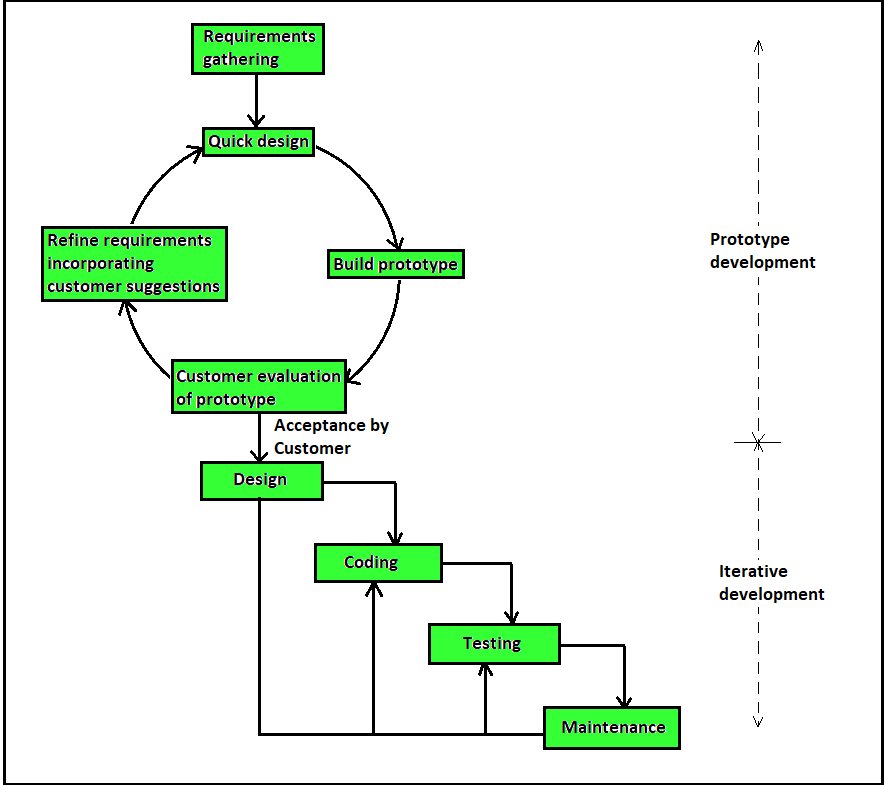
\includegraphics[width=\linewidth]{./Prototyping-model}
		\caption{Prototype Model, Source: \citet{Kumar:2020}}
		\label{fig: 1}
	\end{subfigure}
	\hfill
	\begin{subfigure}[b]{0.45\textwidth}
		\centering
		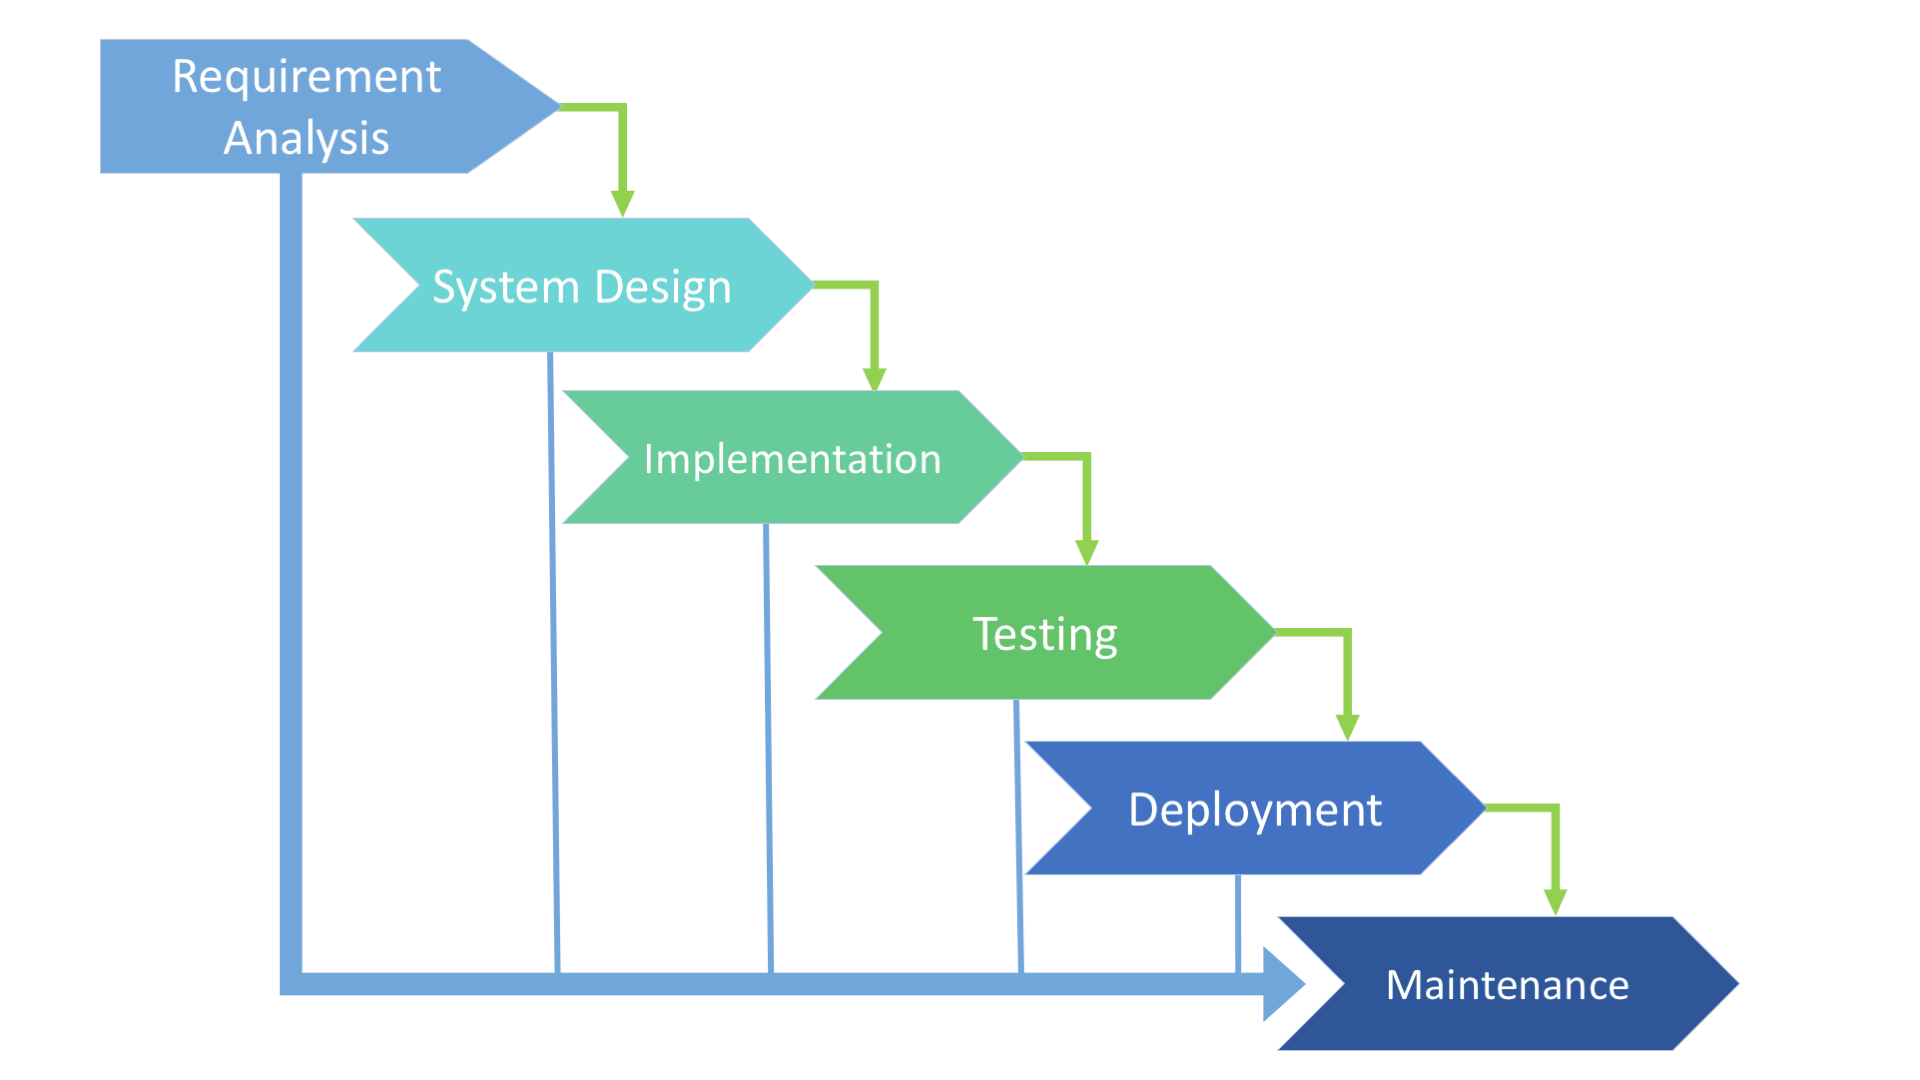
\includegraphics[width=\linewidth]{./waterfall}
		\caption{Waterfall model, Source: \citet{Team:2017}}
		\label{fig: 2}
	\end{subfigure}
	\medskip
	\begin{subfigure}[b]{0.45\textwidth}
		\centering
		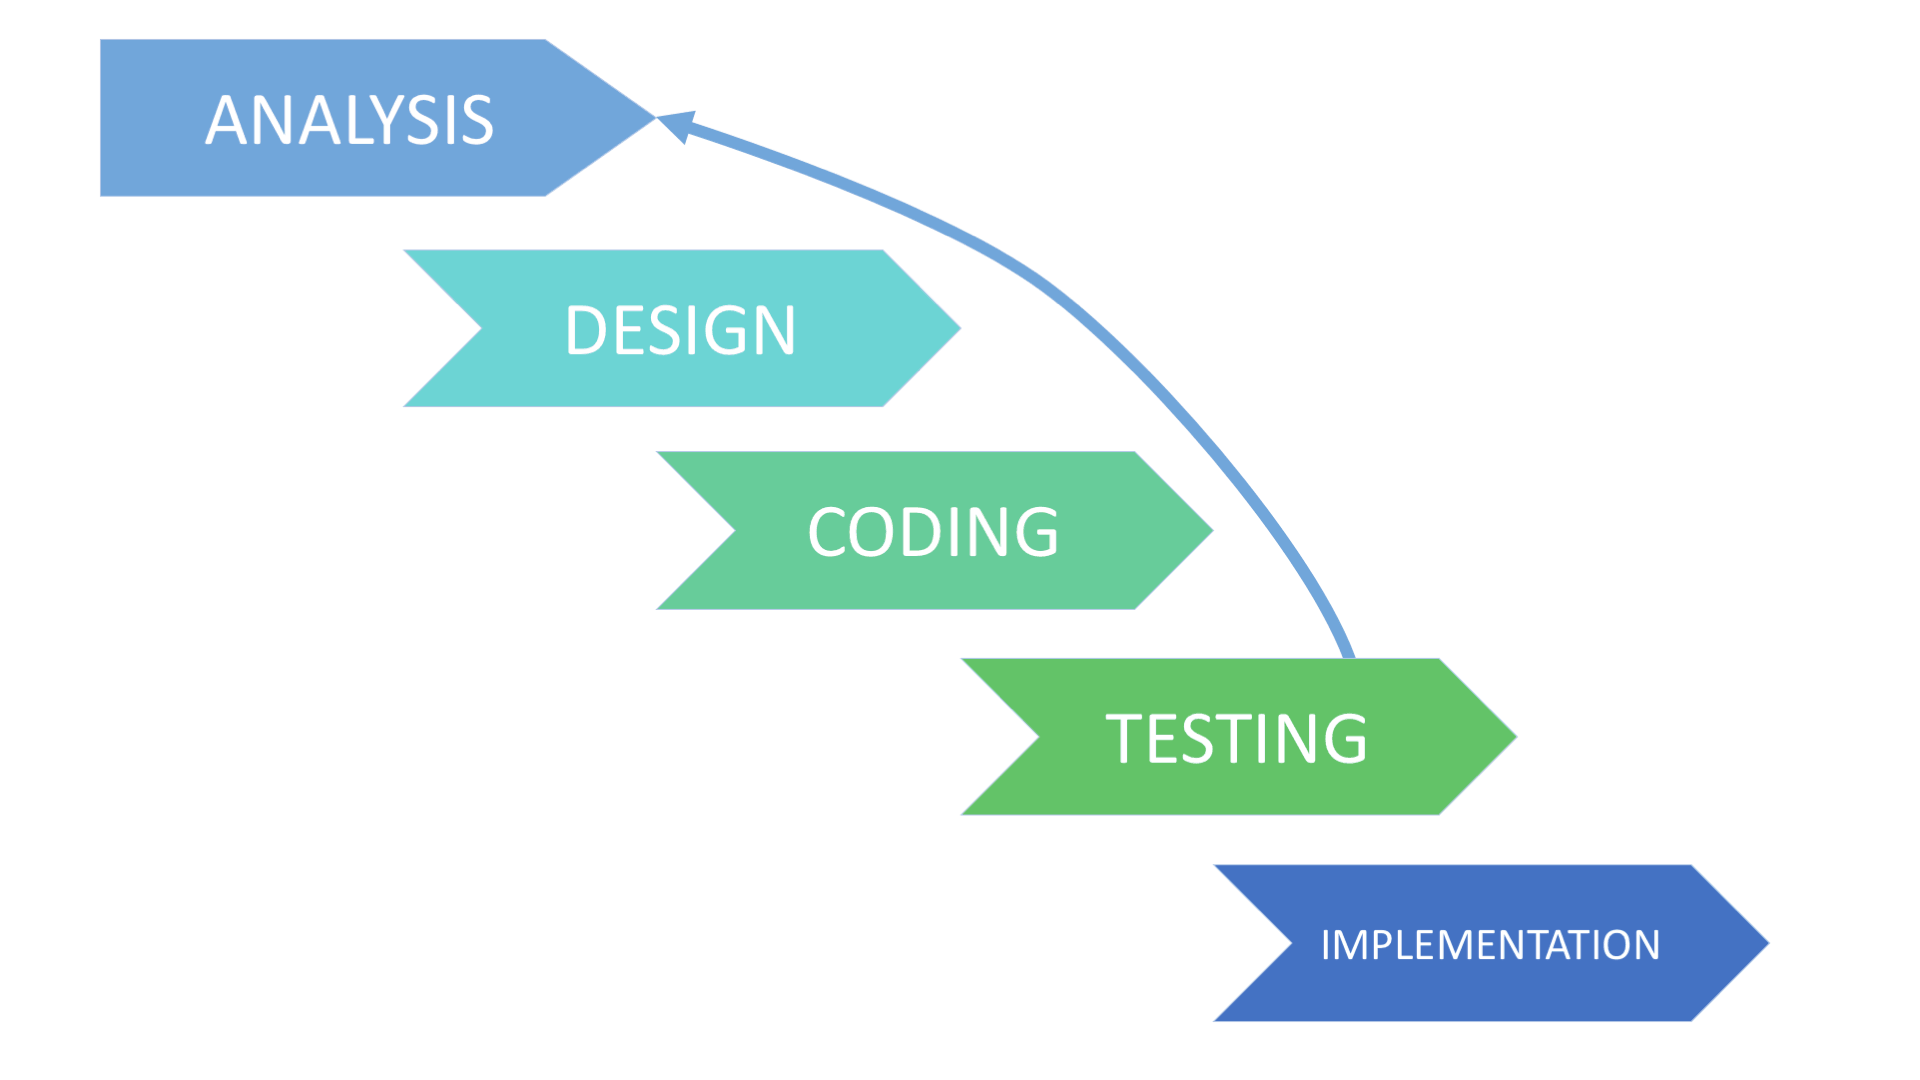
\includegraphics[width=\linewidth]{./iterative}
		\caption{Incremental model, Source: \citet{Team:2017}}
		\label{fig: 3}
	\end{subfigure}
	\hfill
	\begin{subfigure}[b]{0.45\textwidth}
		\centering
		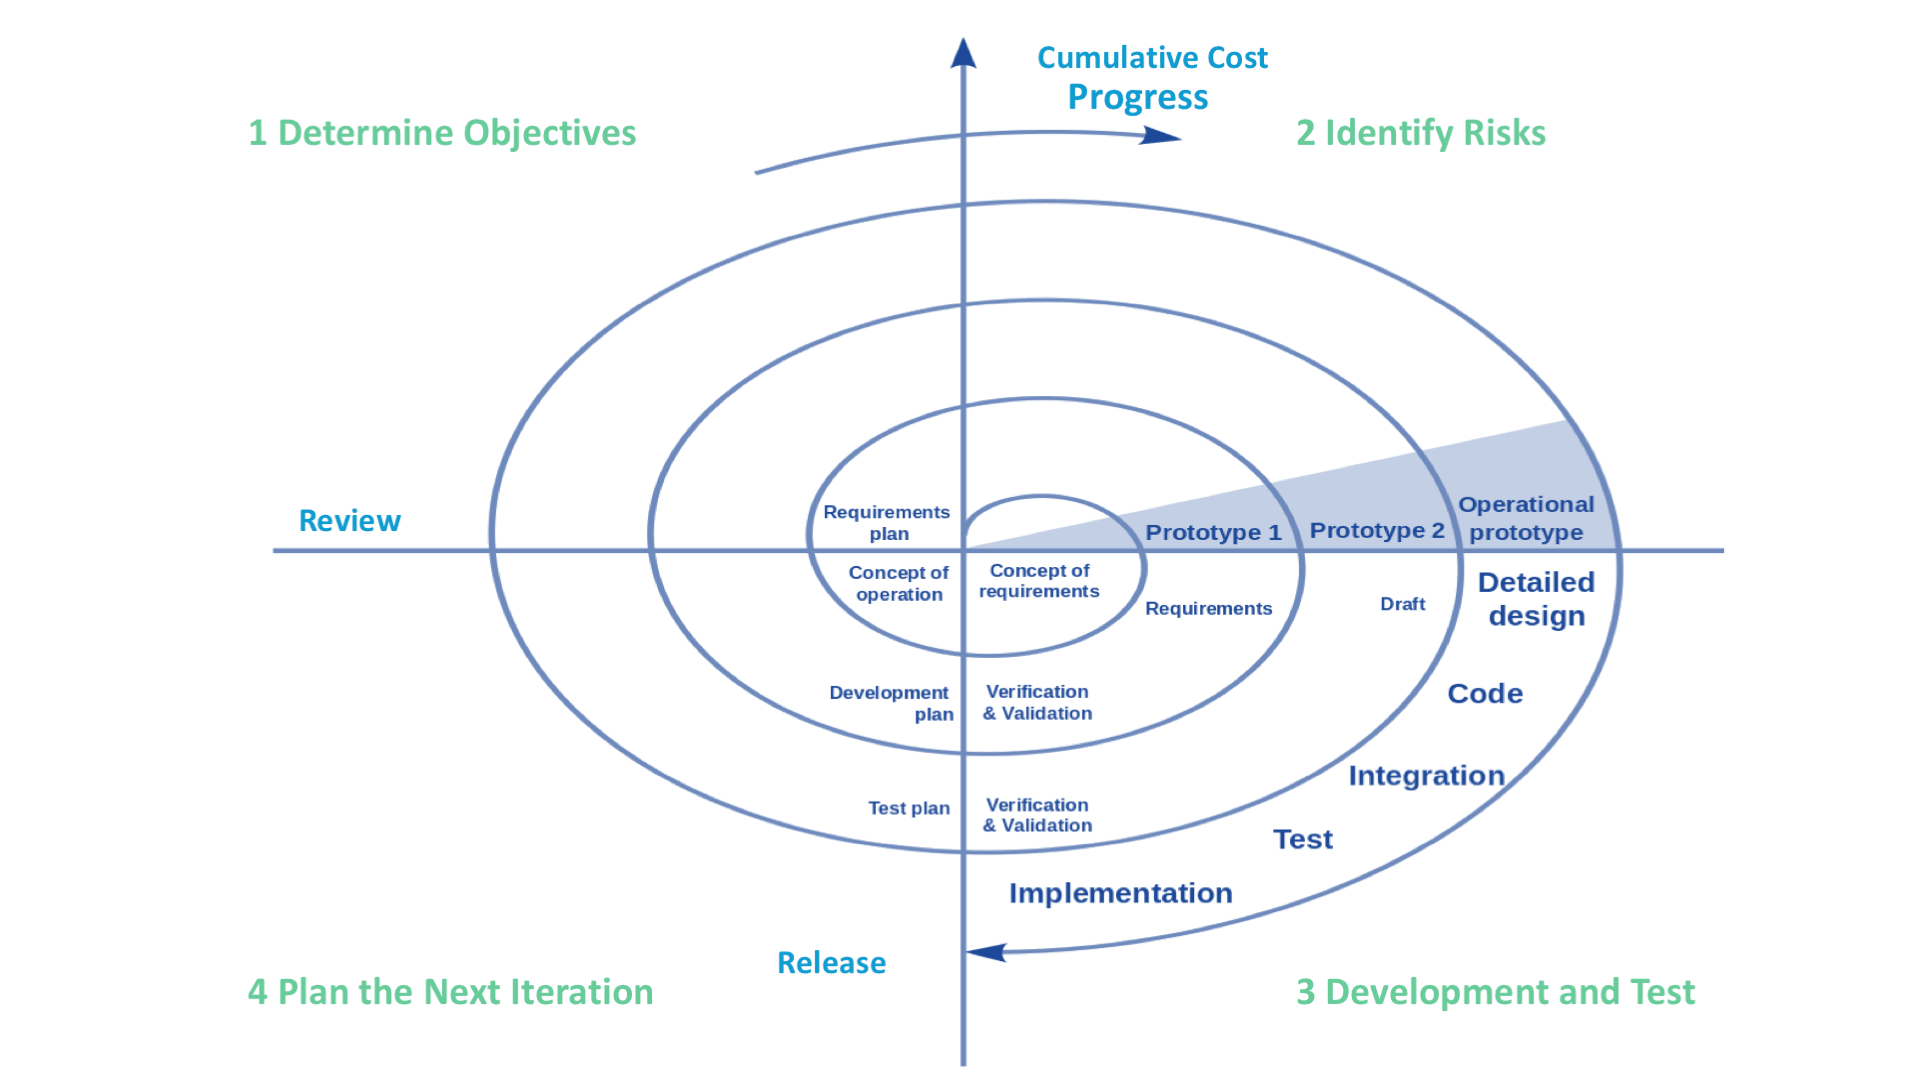
\includegraphics[width=\linewidth]{./Spiral}
		\caption{Spiral model, Source: \citet{Team:2017}}
		\label{fig: 4}
	\end{subfigure}
	\medskip
	\begin{subfigure}[b]{0.45\textwidth}
		\centering
		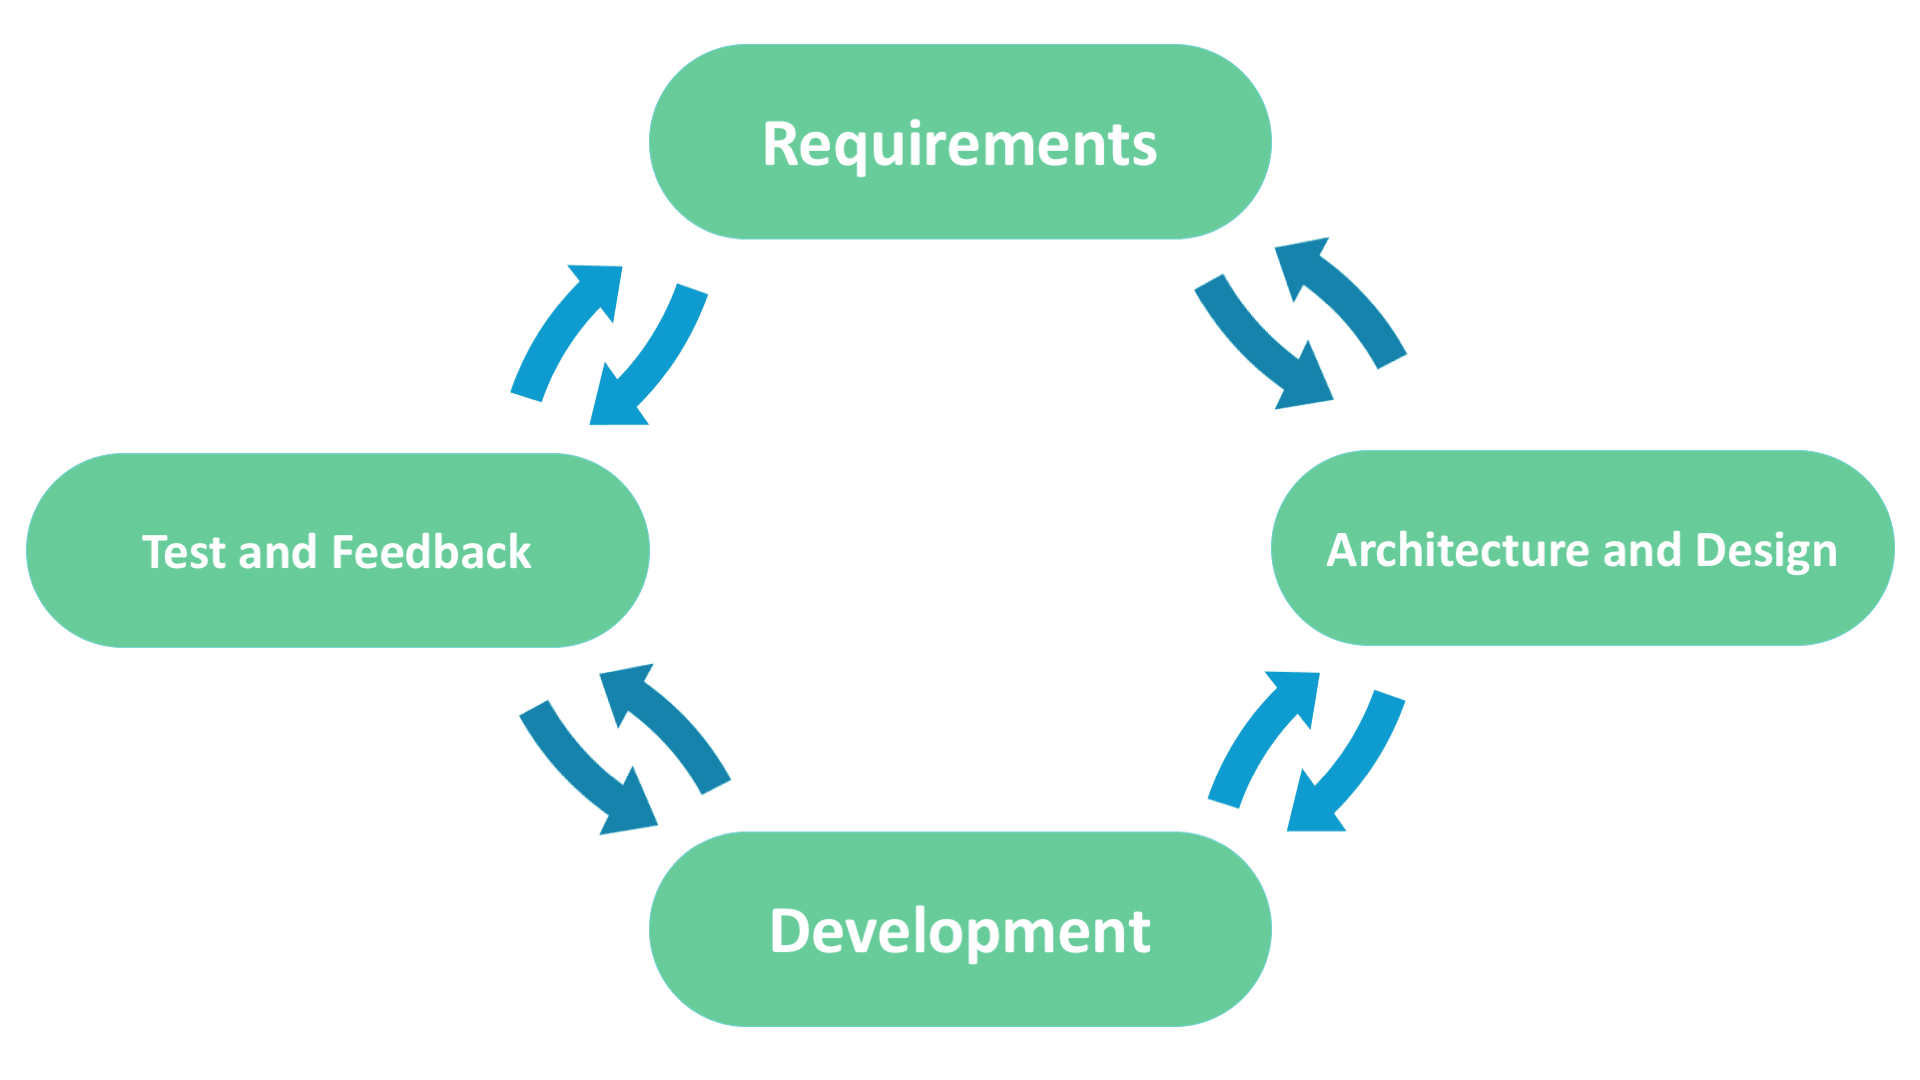
\includegraphics[width=\linewidth]{./Agile}
		\caption{Agile model, Source: \citet{Team:2017}}
		\label{fig: 5}
	\end{subfigure}
	\hfill
	\begin{subfigure}[b]{0.45\textwidth}
		\centering
		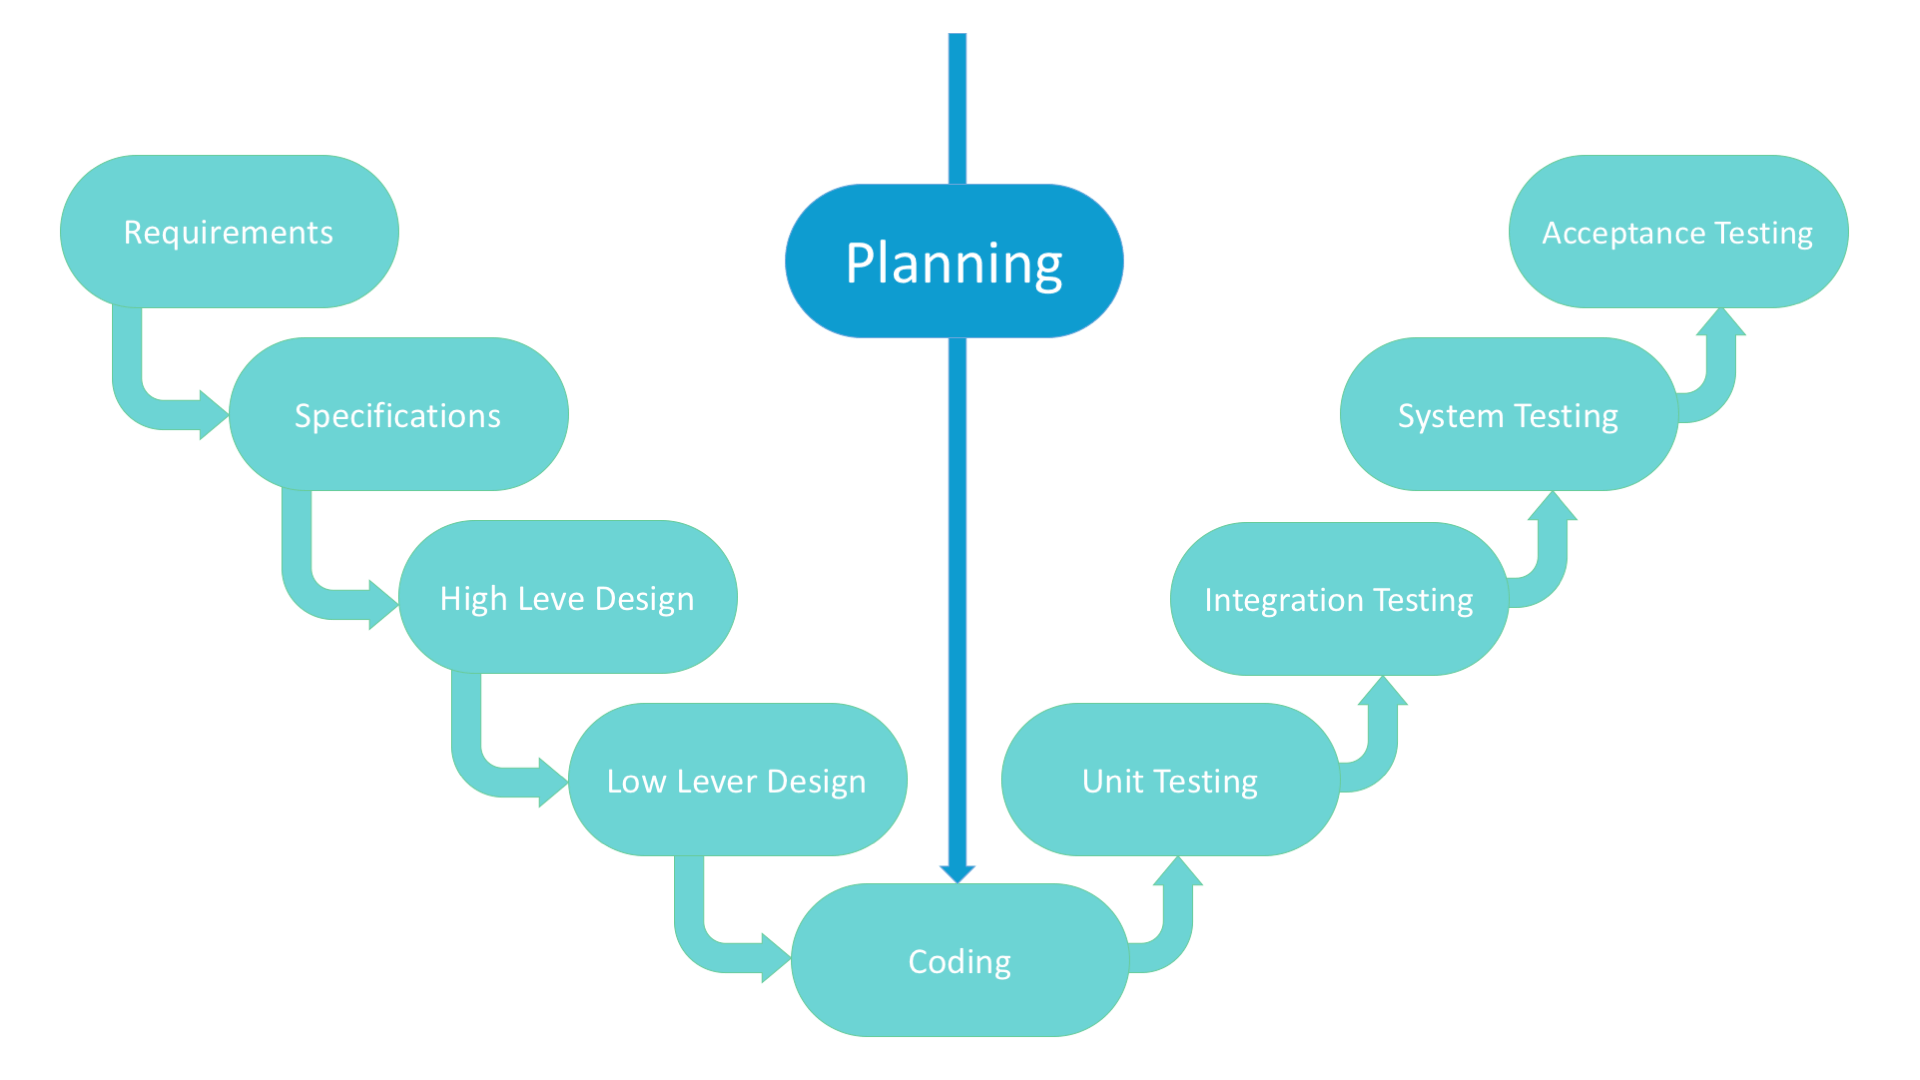
\includegraphics[width=\linewidth]{./V-Shaped}
		\caption{V-shaped model, Source: \citet{Team:2017}}
		\label{fig: 6}
	\end{subfigure}
	\medskip
	\begin{subfigure}[b]{0.5\textwidth}
		\centering
		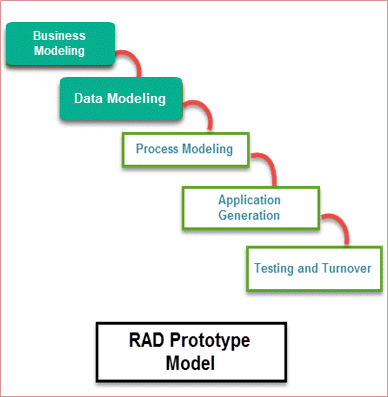
\includegraphics[width=\linewidth]{./rad}
		\caption{Rapid application development model (RAD)}
		\label{fig: 7}
	\end{subfigure}
\caption{\ac{SDLC} Models}
\end{figure}
\subsubsection{Comparison of \ac{SDLC} Models}
Table: 3.1 compares the General software process models on different Parameters as listed and compared in \citet{Sharma:2015}.
\begin{table}[htbp]
	\caption{ Comparison of various \ac{SDLC} Models on different Parameters}
	\label{Table: 3.1}
	\resizebox{\columnwidth}{!}{\begin{tabular}{l l l l l l l l}
		\toprule
		\textbf{Model/Features} & \textbf{Waterfall} & \textbf{Prototype}& \textbf{RAD} & \textbf{Incremental} & \textbf{Spiral} & \textbf{Build \& Fix} & \textbf{V-shaped}\\
		\midrule
		Well defined requirements & Yes & No & Yes & No & No & No & Yes\\
		User involvement in all phases & Only at beginning & High & Only at beginning & Yes(Intermediate) & High & No & No\\
		Risk analysis & Only at beginning & No Risk analysis & Low & No Risk analysis & Yes & No & Only at beginning\\
		Overlapping phases & No overlapping & Yes & No & No & Yes & Yes & No\\
		Implementation time & Long & Quick & Quick & Long & Long & Depend upon Project & Long\\
		Cost & Low & High & Low & Low & Expensive & Low & Expensive\\
		Incorporation of changes & Difficult & Easy & Easy & Easy & Easy & Difficult & Difficult\\
		Simplicity & Simple & Simple & Simple & Intermediate & Intermediate & Simple & Intermediate\\
		Flexibility & Rigid & Little flexible & High & Less flexible & Flexible & FLexible & Less flexible\\
		\bottomrule
	\end{tabular}}
\end{table}
\subsection{Python}
Python is the programming language in which Django and Flask frameworks, used in implementing majority of the projects, were written. It is a general-purpose, versatile and modern programming language with a dynamic scripting ability similar to Perl and Ruby. First released in 1991 by its principal author, Guido van Rossum, Python supports dynamic typing and has a garbage collector for automatic memory management. Another important feature of Python is dynamic name solution which binds the names of functions and variables during execution, \citet{Zhou:2010}.
\subsection{Flask Framework}
Flask is a lightweight \ac{WSGI} web application framework(\citet{Ronacher:2010}) written in Python by Armin Ronacher and first released on the 1st of April, 2010.  It was designed as an extensible framework from the ground up providing a solid core with the basic services while allowing extensions to provide the rest. Since one can pick and choose the required
extension packages, a lean stack with no bloat and which
does exactly what one needs is ended up with.


Flask has two main dependencies, namely \href{http://werkzeug.pocoo.org/}{Werkzeug} and \href{http://jinja.pocoo.org/}{Jinja2}. \href{http://werkzeug.pocoo.org/}{Werkzeug} provides the routing, debugging, and \ac{WSGI} subsystems, while template support is provided by \href{http://jinja.pocoo.org/}{Jinja2} \citet{Grinberg:2014}.
\subsection{Django Framework}
Django is a powerful Python web application framework that encourages rapid development with clean, and pragmatic design, which offers a relatively shallow learning curve, \citet{Antonio:2018}. It is open source with the primary goal of making the development of complex and data-based websites easier. Thus it emphasizes the re-usability and pluggability of components to ensure rapid developments, \citet{Zhou:2010}. Django consists of three layers, namely model, view and template, \citet{Adrian:2019}.
\subsubsection{Model Layer}
Model, the single and definitive source of information about a data, contains the essential fields and behaviors of the data being stored. Generally, each model maps to a single database table, \citet{Adrian:2019}.
\subsubsection{View Layer}
Django's "views", which can be function- or class-based, encapsulate the logic that is responsible for processing a user’s request and for returning the desired response, \citet{Adrian:2019}. Response may be an \ac{HTML} content, \ac{XML} document or error code such as error 404, 505 and so on. The logic encapsulated in a view is allowed to be arbitrary provided that the desired response is returned.
\subsubsection{Template Layer}
The template layer provides a designer-friendly syntax for rendering the information to be presented to the user. A template contains the static parts of the desired \ac{HTML} output as well as some special syntax
describing how dynamic content will be inserted and A Django project can be configured with one or several template engines or systems such as the \ac{DTL} and \href{http://jinja.pocoo.org/}{Jinja2}.
\subsection{\ac{AJAX}}
\ac{AJAX}, a term coined in 2005 by Jesse James Garrett, stands for Asynchronous JavaScript and \ac{XML} and refers to a set of web development techniques combining existing web technologies, including \ac{HTML} or \ac{XHTML}, Cascading Style Sheets, JavaScript, The Document Object Model, \ac{XML}, \ac{XSLT}, and most importantly the \ac{XHR} object, \citet{Yang:2020}. Ajax is widely used in client-side programming (e.g. JavaScript) to allow for data to be sent and received to and from a database or server without actually disturbing the user experience or reloading the entire browser page. Figure 3.2 compares the conventional method of requesting data from a web server and the Ajax method.
\begin{figure}[!htbp]
	\centering
	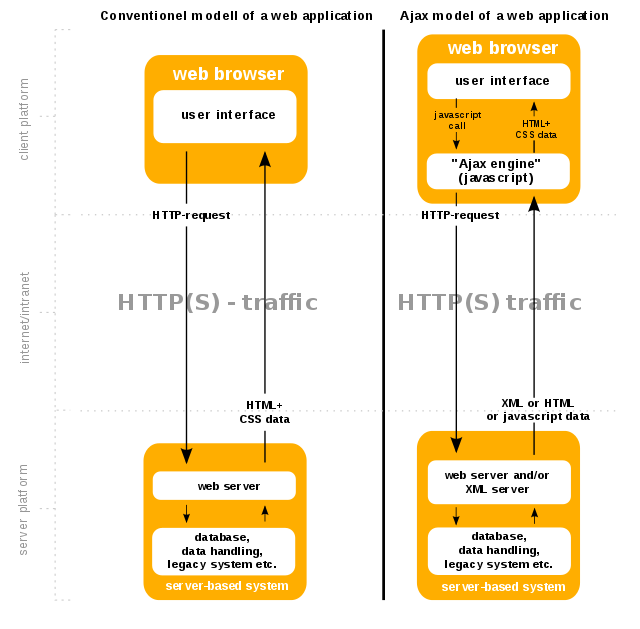
\includegraphics[width=1\textwidth]{./Ajax.png}
	\caption{Conventional method vs \ac{AJAX} method, Source \href{https://en.wikipedia.org/wiki/File:Ajax-vergleich-en.svg}{Wikipedia.com}}
\end{figure}

\ac{AJAX} was greatly utilized in carrying out my projects since most of them exhibited Real-time functionality. Code Snippet 3.1 is a sample snippet from one of the projects with asynchronous data persistence.\\\\\\\\
\begin{code}
	\captionof{listing}{Django Blog's \ac{AJAX} snippet}
	\begin{minted}
	[
	frame=lines,
	framesep=2mm,
	baselinestretch=1,
	fontsize=\footnotesize,
	linenos
	]
	{JavaScript}
$(document).ready(function(event) {
	$(document).on('submit', '#postcomment', function(event) {
	event.preventDefault();
	$.ajax({
		type: 'POST',
		url: $(this).attr('action'),
		data: $(this).serialize(),
		dataType: 'json',
		success: function(response) {
			$('.comments-wrap').html(response['form']);
				$(document).ready(function() {
					$("#commenters").on("click", ".reply",
					function(event) {
						event.preventDefault();
						var form = $("#postcomment").clone(true);
						form.find('.parent').val($(this)
							.parent().parent().attr('id'));
						$(this).parent().append(form).fade();
				});
			});
			$(document).ready(function() {
				var ssPrettyPrint = function() {
					$('pre').addClass('prettyprint');
					$('code').addClass('prettyprint');
					$(document).ready(function() {
						PR.prettyPrint();
					});
				};
			});
		},
		error: function(rs, e) {
			console.log(rs.responseText);
		},
	})
});
});	
	\end{minted}
\end{code}

The above snippet was the underlying code responsible for the real-time functionality of Django blog's commenting system. It updates and fetches data from the Comment table which had been created in the blog's models without reloading the entire web page.
\subsection{SQLAlchemy}
According to \citet{Bayer:2016}, The SQLAlchemy \ac{SQL} Toolkit and \ac{ORM} provide a comprehensive set of tools for working with databases and Python. It consists of several distinct areas of functionality which can be individually or collaboratively used together. Below is the illustration of the major components of SQLAlchemy, with component dependencies organized into layers:
\begin{figure}[htbp]
	\centering
	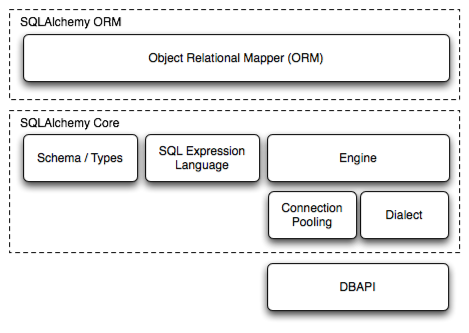
\includegraphics[width=1\textwidth]{./sqlalchemy.png}
	\caption{SQLAlchemy overview, from \citet{Bayer:2016}}
\end{figure}


From the above figure, the two most significant front-facing portions of SQLAlchemy are the \ac{ORM} and the \ac{SQL} Expression Language. SQL Expressions can be used independently of the \ac{ORM}. When using the \ac{ORM}, the \ac{SQL} Expression language remains part of the public facing \ac{API} as it is used within object-relational configurations and queries, \citet{Bayer:2016}.
\subsection{\href{http://jinja.pocoo.org/}{Jinja2}}
\href{http://jinja.pocoo.org/}{Jinja2} is a fast, expressive, extensible and modern day web templating language or engine for Python developers mimicking \ac{DTL} with the inclusion of call functions with arguments on objects. From \citet{Ronacher:2017}, An important usage of Jinga2 is the creation of \ac{HTML}, \ac{XML} or other markup formats which are returned to the user via \ac{HTTP} response.
\section{Python-based Projects}
\subsection{Methodology}
All of the web applications were built using Flask or Django framework at the Back-end and Creative Tim's dashboard and other extensible templates at the front-end following the procedures below:
\subsubsection{Created the Database tables}
To get started, a back-end of the system which is the database was created. It should be noted that the implementation of this system is framework dependent as discussed below.
\begin{itemize}
	\item \textbf{Flask}: One of the notable tables in the database was the User table which was created by writing a Class that inherited from Flask's model class. A snippet is as follows:

	\begin{code}
	\captionof{listing}{\ac{vCPE} Flask User Model}
	\begin{minted}
		[
		frame=lines,
		framesep=2mm,
		baselinestretch=1,
		fontsize=\footnotesize,
		linenos
		]
	{python}
from app         import db
from flask_login import UserMixin

from . common    import COMMON, STATUS, DATATYPE

class User(UserMixin, db.Model):

	id          = db.Column(db.Integer,     primary_key=True)
	user        = db.Column(db.String(64),  unique = True)
	email       = db.Column(db.String(120), unique = True)
	name        = db.Column(db.String(500))
	role        = db.Column(db.Integer)
	password    = db.Column(db.String(500))
	password_q  = db.Column(db.Integer)

	def __init__(self, user, password, name, email):
		self.user       = user
		self.password   = password
		self.password_q = DATATYPE.CRYPTED
		self.name       = name
		self.email      = email
		self.group_id = None
		self.role     = None

	def __repr__(self):
		return '<User %r>' % (self.id)

	def save(self):

		# inject self into db session    
		db.session.add ( self )

		# commit change and save the object
		db.session.commit( )

		return self 
	\end{minted}
	\end{code}
	This piece of code creates a table called \texttt{User} which stores the user information. The table has seven columns: \texttt{id}, a primary key; \texttt{user}  which corresponds to \texttt{User}'s username; \texttt{email} corresponding to \texttt{User}'s email; \texttt{name} corresponding to the name of the \texttt{User}; role; \texttt{password} and \texttt{password\_q} corresponding to the password and confirm password fields respectively of the \texttt{User}. There are also the \texttt{\_\_init\_\_}(Python's Object constructor), \texttt{\_\_repr\_\_}, and \texttt{save} methods all taking \texttt{\textit{"self"}} as argument, a requirement in Python programming language for methods. \texttt{\_\_init\_\_} and \texttt{\_\_repr\_\_} are called \textit{dunder} or Double Under(Underscores) methods which are some times referred to as Magic methods. When an object of the class \texttt{User} is created, the \texttt{\_\_init\_\_} method is invoked while \texttt{\_\_repr\_\_} as well as its counterpart, \texttt{\_\_str\_\_}, found in Code Snippet 3.2 line 31, controls the \texttt{to-string} conversion in the class that houses it.

	
	It is worth noting that Flask uses \texttt{SQLAlchemy} for the \ac{ORM} or Data Access part. It takes charge of the database management such as creating tables, writing \ac{SQL} queries and other database operations. 
	
	
	\item \textbf{Django}: For Django, creation of tables is fairly more verbose but simple. The snippet below buttresses this point.
		\begin{code}
		\captionof{listing}{Django Blog's PublishedManager, Category,and Post}
	\begin{minted}
		[
		frame=lines,
		framesep=2mm,
		baselinestretch=1,
		fontsize=\footnotesize,
		linenos	
		]
		{python}
from django.contrib.postgres.fields import ArrayField
from django.db import models
from django.contrib.contenttypes.models import ContentType
from django.contrib.auth.models import User
from ckeditor_uploader.fields import RichTextUploadingField
from ckeditor.fields import RichTextField
from django.utils import timezone
from django.urls import reverse
from django.db.models.signals import pre_save
from PIL import Image
from taggit.managers import TaggableManager
from .utils import get_read_time
from django.utils.safestring import mark_safe
#from django.contrib.contenttypes.fields import GenericRelation
		
# Create your models here.
		
class PublishedManager(models.Manager): 
	def get_queryset(self): 
		return super(PublishedManager, self).get_queryset()
		.filter(status='published')
		
class Category(models.Model):
	name = models.TextField(max_length=1000000)
	slug = models.SlugField(max_length=10000000, unique=True)
		
	class Meta:
		ordering = ('name',)
		verbose_name='category'
		verbose_name_plural = 'categories'
		
	def __str__(self):
		return self.name
		
class Post(models.Model):
	STATUS_CHOICES = ( 
		('draft', 'Draft'), 
		('published', 'Published'), 
	) 
	title   = models.CharField(max_length=10000000) 
	slug    = models.SlugField(max_length=10000000, unique_for_date='publish') 
	author  = models.ForeignKey(User, on_delete=models.CASCADE,
	related_name='blog_posts')
	image   = models.ImageField(upload_to='posts_pics'
	,default='logo.svg')
	body    = RichTextUploadingField()
	publish = models.DateTimeField(default=timezone.now)
	read_time =  models.IntegerField(default=0)  
	created = models.DateTimeField(auto_now_add=True) 
	updated = models.DateTimeField(auto_now=True) 
	status  = models.CharField(max_length=100
	,choices=STATUS_CHOICES, default='draft') 
	objects = models.Manager() # The default manager. 
	published = PublishedManager() # Our custom manager.
	category = models.ForeignKey(Category, on_delete=models.CASCADE)
	tags = TaggableManager()
	class Meta: 
		ordering = ('-created',) 
		
	def __str__(self): 
		return self.title
		
		
	def get_absolute_url(self):
		return reverse('blog:post_detail',args=[self.publish.year
		, self.publish.month, self.publish.day, self.slug])
		
	def get_next_post(self):
		return self.get_next_by_created()
		
	def get_previous_post(self):
		return self.get_previous_by_created()
		
	def get_markdown(self):
		body = self.body
		return mark_safe(body)
		
	@property
	def get_content_type(self):
		instance = self
		content_type = ContentType.objects.get_for_model(instance.__class__)
		return content_type
		
	def save(self, *args, **kwargs):
		super(Post, self).save(*args, **kwargs)
		
		img = Image.open(self.image.path)
		width = 883
		height = 391
		if img.width > width or img.height > height:
			output_size = (width, height)
			img.thumbnail(output_size)
			img.save(self.image.path)
	\end{minted}
\end{code}
\end{itemize}
\subsubsection{Created the User Interface}
Although the Database, where tables of any kind could be updated using Django and/or Flask models, had been created, it would be a disaster for users and the technical maintenance team if end users are allowed to manipulate the data directly. Therefore, nice and responsive user interfaces were created to let users interact with the data indirectly. As discussed above, Flask and Django provide templating components to create the user interfaces. Since Flask solely uses \href{http://jinja.pocoo.org/}{Jinja2} whereas Django has an optional \ac{DTL}, the syntax for creating the user interfaces are a bit different.
\begin{itemize}
	\item \textbf{Django}: Django supports two templating engines, namely \href{http://jinja.pocoo.org/}{Jinja2} and \ac{DTL} where the latter happens to be the default with the below snippet.
	\begin{code}
		\captionof{listing}{Django Blog's \texttt{post\_form.html}}
		\begin{minted}
			[
			frame=lines,
			framesep=2mm,
			baselinestretch=1,
			fontsize=\footnotesize,
			linenos
			]
			{HTML}



<!-- site content
================================================== -->
<div class="s-content content">
	<main class="row content__page">
		<section class="column large-full entry format-standard">
			<div class="content__page-header">
				<h1 class="display-1">
					Write A Post.
				</h1>
			</div> <!-- end content__page-header -->
			<form name="contactForm" id="contactForm" method="post"
			action="" autocomplete="on" enctype="multipart/form-data">
				
				<fieldset>
					
						<div class="form-field">
							{{ form.media }}
							{{ field.label }}
							{{ field }}
						</div>
					
					<input name="submit" id="submit" class="btn
					btn--small" value="Create Post" type="submit">
				</fieldset>
			</form> <!-- end form -->
		</section>
	</main>
</div> <!-- end s-content -->

		\end{minted}
	\end{code}
Every line surrounded by \texttt{"\% \%"} is a Django sentence which deals with simple \texttt{"if-else"}, \texttt{csrf\_token} and \texttt{"for-loop"} among others. The lines surrounded by double curly braces, such as \texttt{\{\{ field \}\}}, denote variables whose values are passed from view functions whenever this template has to be displayed.

	\item \textbf{Flask}: For flask, \href{http://jinja.pocoo.org/}{Jinja2} is one of the major dependencies needed to get it up and running and the syntax looks as follows:
	\begin{code}
		\captionof{listing}{CEA Dashboard \texttt{login.html}}
		\begin{minted}
[
frame=lines,
framesep=2mm,
baselinestretch=1,
fontsize=\footnotesize,
linenos
]
{HTML}
<!DOCTYPE html>
<html lang="en">
<head>
<meta charset="UTF-8">
<meta name="viewport" content="width=device-width, initial-scale=1">

	<title>ipNX dashboard - {{ title }}</title>

	<title>ipNX dashboard</title>

</head>
<body>
	<div class="limiter">
		<div class="container-login100">
			<div class="wrap-login100">
				<form class="login100-form validate-form"
				method="POST" action="">
					{{ form.hidden_tag() }}
					<span class="login100-form-logo">
						<img
							src="/static/assets/custom/login
							/images/logo.png" alt="">
					</span>
					<span class="login100-form-title p-b-34 p-t-27">
						Log in
					</span>
					
						<div class="text-center p-t-5 p-b-5">
							<p class="error">
								{{ message }}
							</p>      
						</div>
					
					<div class="wrap-input100 validate-input"
					data-validate="Enter E-mail">
						{{ form.email(class="input100",
							placeholder="E-mail") }}
						<span class="focus-input100"
							data-placeholder="&#xf207;">
						</span>
					</div>
			
					<div class="wrap-input100 validate-input"
					data-validate="Enter password">
						{{ form.password(placeholder="Password",
							class="input100") }}
							<span class="focus-input100"
								data-placeholder="&#xf191;">
							</span>
					</div>
			
					<div class="contact100-form-checkbox">
						{{ form.remember(class="input-checkbox100",
							id="ckb1",type="checkbox") }}
						<label class="label-checkbox100" for="ckb1">
							Remember me
						</label>
					</div>
			
					<div class="container-login100-form-btn">
			
						{{ form.submit(class="login100-form-btn") }}
			
					</div>
			
					<div class="text-center p-t-10">
						<a class="txt1" href="#">
							Forgot Password?
						</a>
					</div>
				</form>
			</div>
		</div>
	</div>
			
</body>
			
</html>
		\end{minted}
	\end{code}
\end{itemize}
\subsection{Implemented the view function}
Having dealt with the back-end databases and the frontend web pages user interfaces, the logic which stands in between to deal with the user requests and maintain the database were implemented. Unsurprisingly, the view systems in Flask and Django are different.
\begin{itemize}
	\item \textbf{Django}: Django's views component provides a set of \ac{API} to implement the logic. The Django view file, \texttt{views.py}, houses the functions and/or classes to achieve all set goals. The view functions and/or classes are shown in the snippet below:
	\begin{code}
		\captionof{listing}{Django's Blog \texttt{views.py}}
		\begin{minted}
[
frame=lines,
framesep=2mm,
baselinestretch=1,
fontsize=\footnotesize,
linenos
]
{python}
from django.shortcuts import render, get_object_or_404, redirect
from django.contrib.contenttypes.models import ContentType
from django.template.defaultfilters import slugify
from django.http import HttpResponse, HttpResponseRedirect, 
Http404, JsonResponse
from django.core.paginator import Paginator, 
EmptyPage, PageNotAnInteger
from django.views import generic
from django.contrib.auth.mixins import LoginRequiredMixin
, UserPassesTestMixin

from taggit.models import Tag
from django.contrib.auth.decorators import login_required
from django.db.models import Count, Q
from django.contrib.auth.models import User
from .models import Post, Comment
from .forms import PostForm, UpdatePostForm, CommentForm
from django.template.loader import render_to_string
from django.contrib.postgres.search import SearchVector, 
SearchQuery, SearchRank, TrigramSimilarity

#Function based view
def blog_index(request, tag_slug=None):
	object_list = Post.published.all()
	if request.user.is_staff or request.user.is_superuser:
		object_list = Post.objects.all()
	common_tags = Post.tags.most_common()[:2]
	tag = None

	if tag_slug:
		tag = get_object_or_404(Tag, slug=tag_slug)
		object_list = object_list.filter(tags__in=[tag])

	paginator = Paginator(object_list, 5) # 5 posts in each page
	page = request.GET.get('page')
	try:
		posts = paginator.page(page)
		except PageNotAnInteger:
		# If page is not an integer deliver the first page
		posts = paginator.page(1)
	except EmptyPage:
		# If page is out of range deliver last page of results
		posts = paginator.page(paginator.num_pages)
	context = {
		'page': page, 
		'posts': posts, 
		'tag': tag, 
		'common_tags': common_tags,
	}
	return render(request, 'blog/index.html', context)
	
#Class based view
class PostUpdateView(LoginRequiredMixin, 
		UserPassesTestMixin, generic.UpdateView):
	model = Post
	form_class=UpdatePostForm
	template_name = 'blog/post_form.html'

	def form_valid(self, form):
		form.instance.author = self.request.user
		return super().form_valid(form)

	def test_func(self):
		post = self.get_object()
	if self.request.user == post.author or self.request.user.is_staff:
		return True
	return False
		\end{minted}
	\end{code}
	\item \textbf{Flask}: According to \citet{Grinberg:2014}, "Clients such as web browsers send requests to the web server, which in turn sends them to the Flask application instance. The application instance needs to know what code needs to run for each URL requested, so it keeps a mapping of URLs to Python functions. The association between a URL and the function that handles it is called a \texttt{route}. The most convenient way to define a route in a Flask application is through the \texttt{app.route} decorator exposed by the application instance, which registers the decorated
	function as a \texttt{route}. The following example shows how a route is declared using this decorator:
	\begin{code}
		\captionof{listing}{Example snippet}
		\begin{minted}
[
frame=lines,
framesep=2mm,
baselinestretch=1,
fontsize=\footnotesize,
linenos
]
{python}
@app.route('/')
def index():
	return '<h1>Hello World!</h1>'

		\end{minted}
	\end{code}
Functions like index() are called view functions" and are mostly housed in the \texttt{views.py} file and an example of a comprehensive \texttt{views.py} file is shown below:
\begin{code}
	\captionof{listing}{An excerpt from CEA dashboard's \texttt{views.py} file}
	\begin{minted}
[
frame=lines,
framesep=2mm,
baselinestretch=1,
fontsize=\footnotesize,
linenos
]
{python}
# all the imports necessary

from flask import json, url_for, redirect, Markup, 
Response, render_template, flash, g, session, jsonify, 
request, send_from_directory
from werkzeug.exceptions import HTTPException, NotFound, abort

import os
import secrets
from PIL import Image
from app  import app

from flask       import url_for, redirect, render_template, 
flash, g, session, jsonify, request, send_from_directory
from flask_login import login_user, logout_user, 
current_user, login_required
from app         import app, lm, db, bc
from . models    import User
from . common    import COMMON, STATUS
from . assets    import *
from . forms     import LoginForm, RegisterForm, UpdateAccountForm
import os, shutil, re, cgi, json, random, time
from datetime import datetime


random.seed()  # Initialize the random number generator

# provide login manager with load_user callback
@lm.user_loader
def load_user(user_id):
	return User.query.get(int(user_id))
@app.route('/index')
@login_required
def index():
	inactiveCustomers = 34546
	activeCustomers = 7654984
	numberOfCalls = 123456
	numberOfRetailCustomers = 455674666
	return render_template('pages/index.html',
	numberOfCalls=numberOfCalls,
	numberOfRetailCustomers=numberOfRetailCustomers,
	inactiveCustomers=inactiveCustomers,
	activeCustomers=activeCustomers)


# authenticate user
@app.route('/logout')
def logout():
	logout_user()
	return redirect(url_for('login'))
	\end{minted}
\end{code}
\end{itemize}

\subsection{Projects Implemented}
\subsubsection{Customer Premises Equipment (CPE)}
\begin{itemize}
	\item \textbf{Project's Requirement specification}:
	The project was to "build a web UI for a customer premises equipment (CPE) through which settings can be modified.
	
	Please design such a web UI with the following pages:
	\begin{itemize}
		\item[*] Login page - username and password
		\item[*] Main page - device summary showing WAN and LAN IPv4 addresses
		\item[*] Settings page -
		\subitem Enable/disable DHCP service, modify address range, manage DHCP reservations
		\subitem Manage DNS servers
		\subitem Manage device whitelist/blacklist based on MAC addresses
		\subitem Manage WiFi settings including ESSID name and pre-shared key (password), enable/disable 2.4GHz and/or 5GHz bands, add or remove WiFi devices
	\end{itemize} 
	
	
	This must be a responsive site with a nice UI and interaction. Communication between front-end and back-end should JSON over XHR asynchronously. Backend should be Python or PHP based with data persistence in SQLite on the backend server".
\end{itemize}

Having implemented the features stated using Flask, the system was initiated and Figure 3.3 shows the pages of each feature:
\begin{figure}[!htbp]
	\centering
\begin{subfigure}[b]{0.45\textwidth}
	\centering
	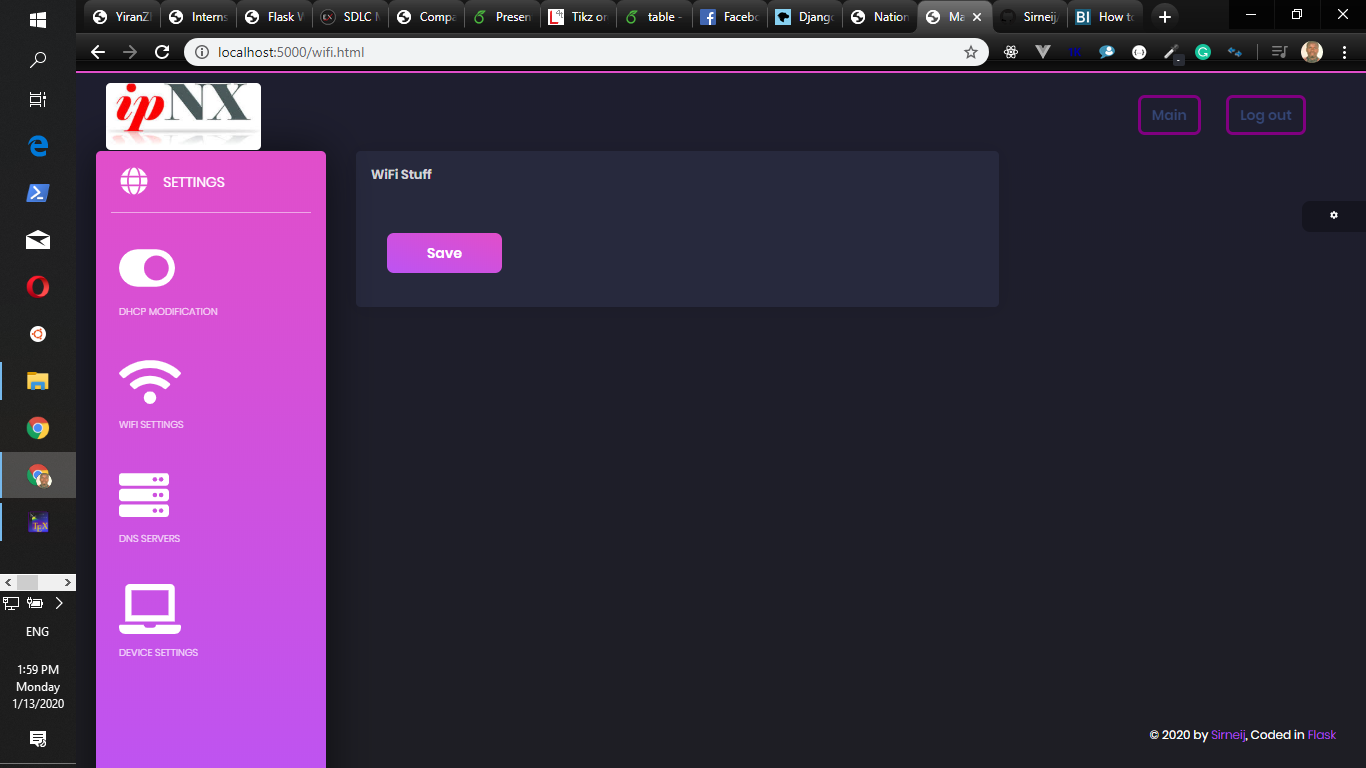
\includegraphics[width=\linewidth]{./vcpewifi}
	\caption{\ac{vCPE} WiFi management page}
\end{subfigure}
\hfill
\begin{subfigure}[b]{0.45\textwidth}
	\centering
	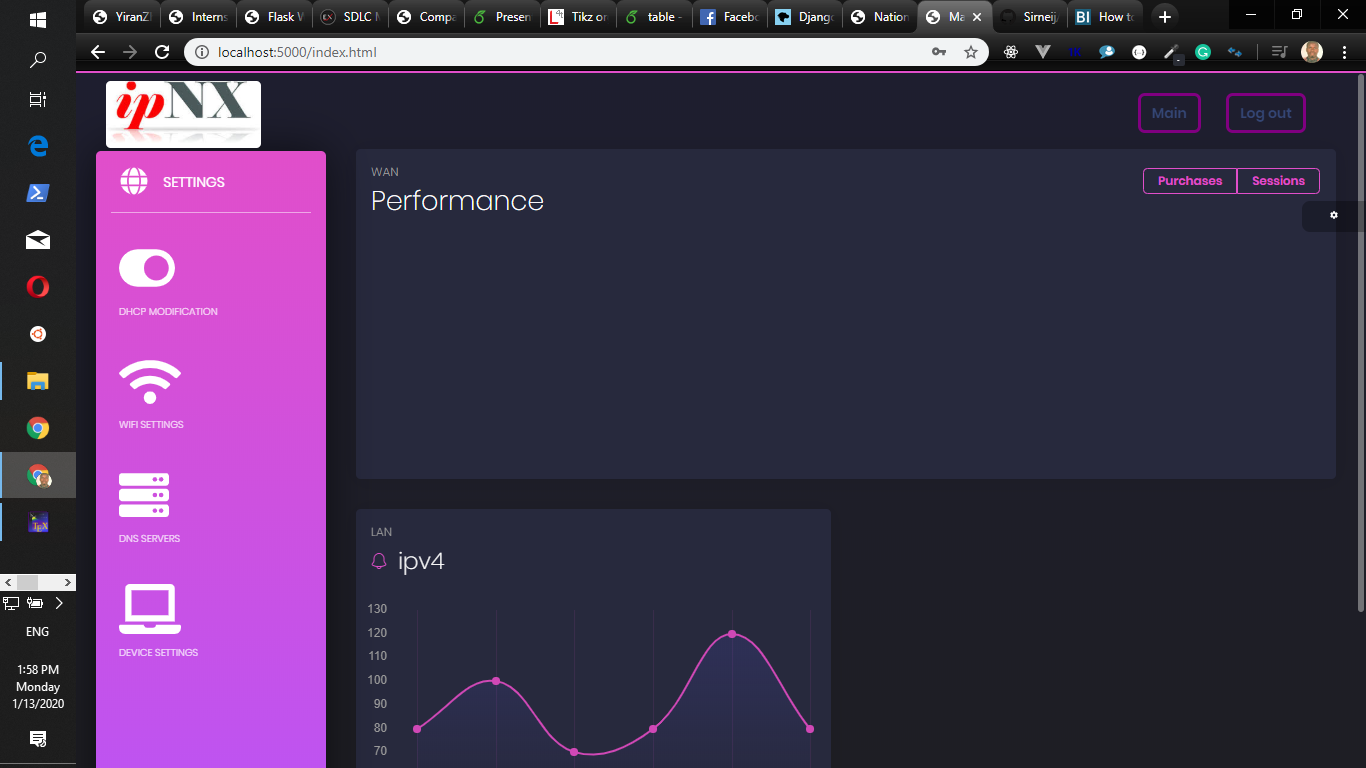
\includegraphics[width=\linewidth]{./vcpemainpage}
	\caption{\ac{vCPE}  Main page}
\end{subfigure}
\medskip
\begin{subfigure}[b]{0.45\textwidth}
	\centering
	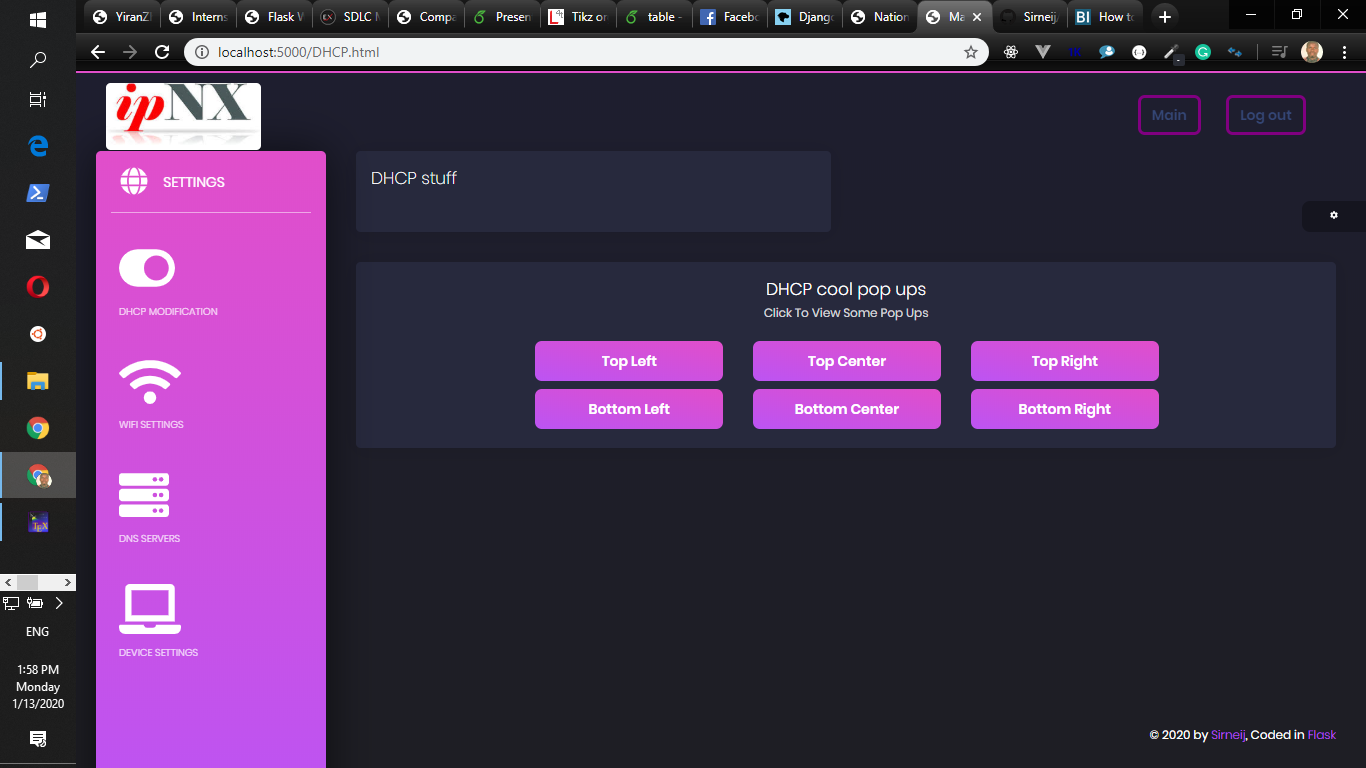
\includegraphics[width=\linewidth]{./vcpedhcp}
	\caption{\ac{vCPE} DHCP page}
\end{subfigure}
\hfill
\begin{subfigure}[b]{0.45\textwidth}
	\centering
	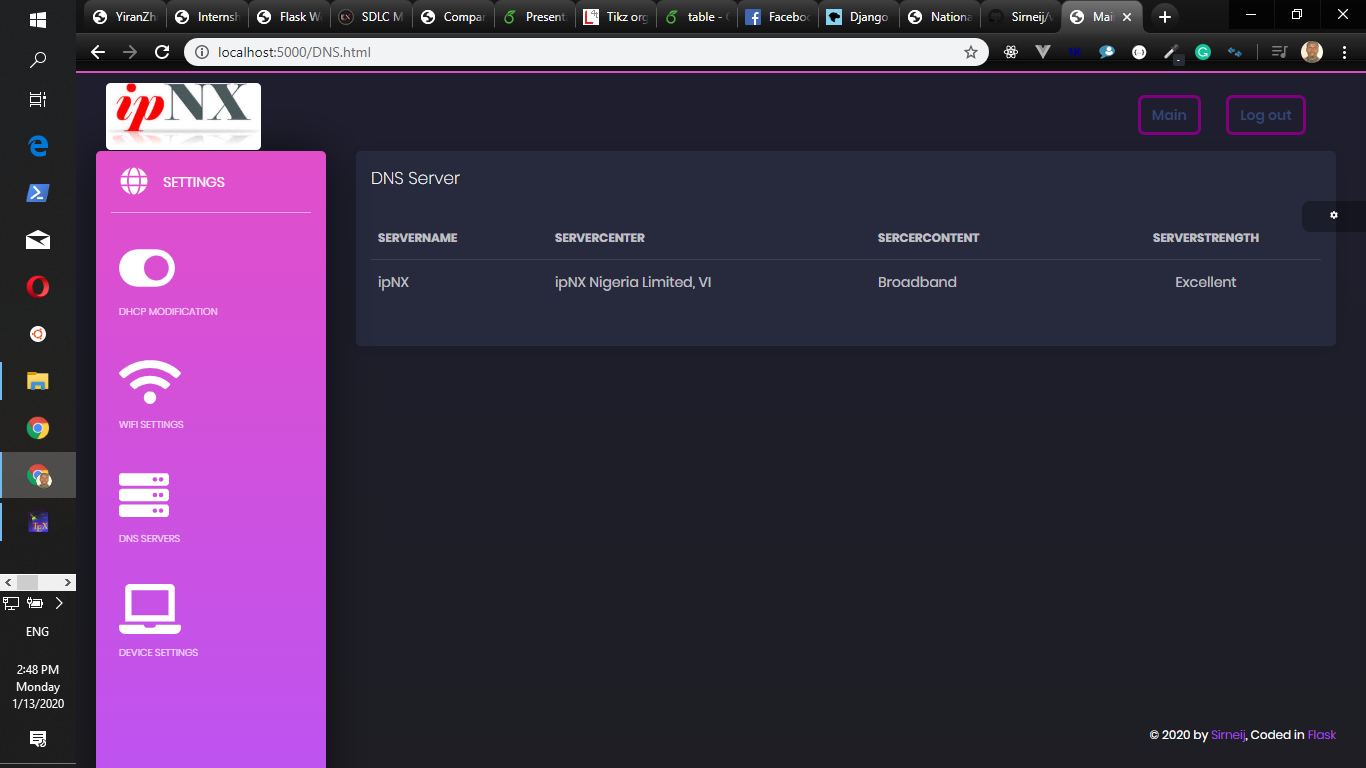
\includegraphics[width=\linewidth]{./vcpednsserver}
	\caption{\ac{vCPE}  DNS Server page}
\end{subfigure}
\medskip
\begin{subfigure}[b]{0.45\textwidth}
	\centering
	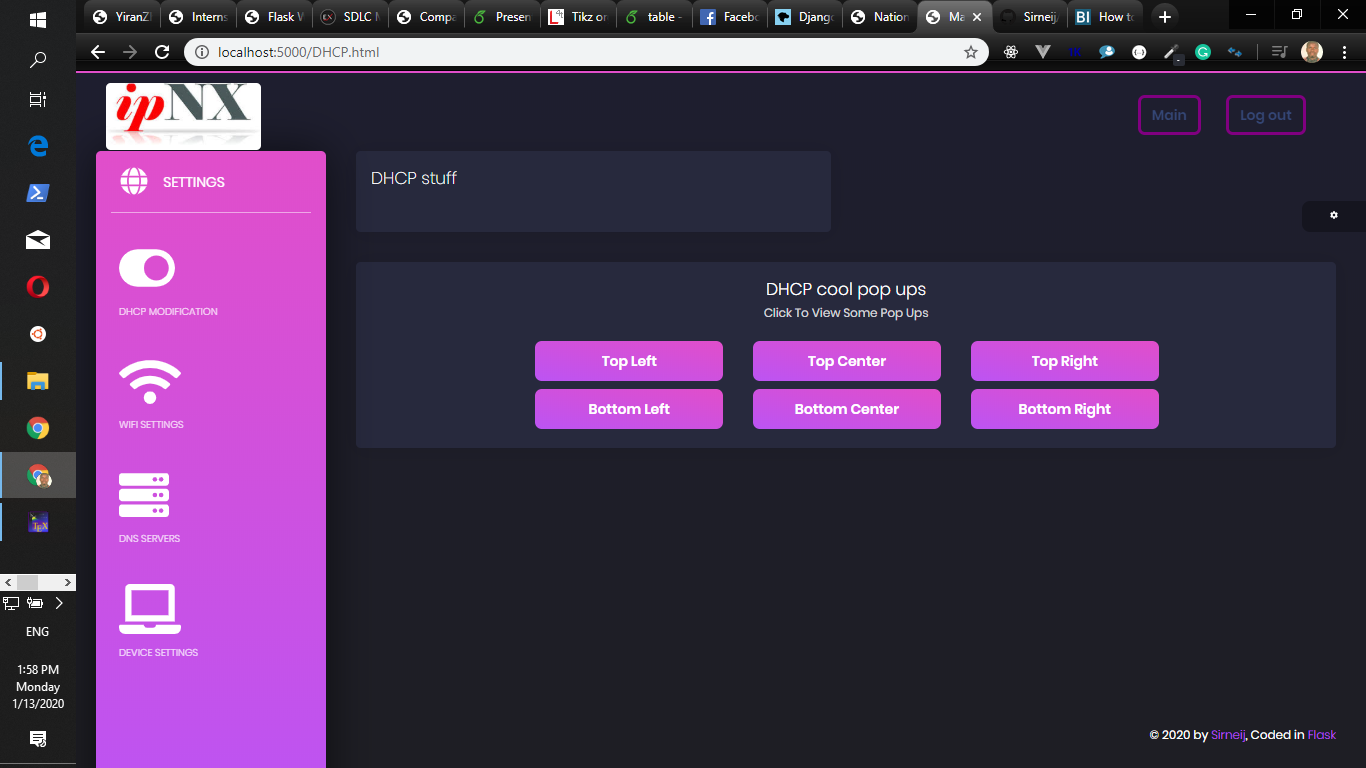
\includegraphics[width=\linewidth]{./vcpedhcp}
	\caption{\ac{vCPE} DHCP page}
\end{subfigure}
\hfill
\begin{subfigure}[b]{0.45\textwidth}
	\centering
	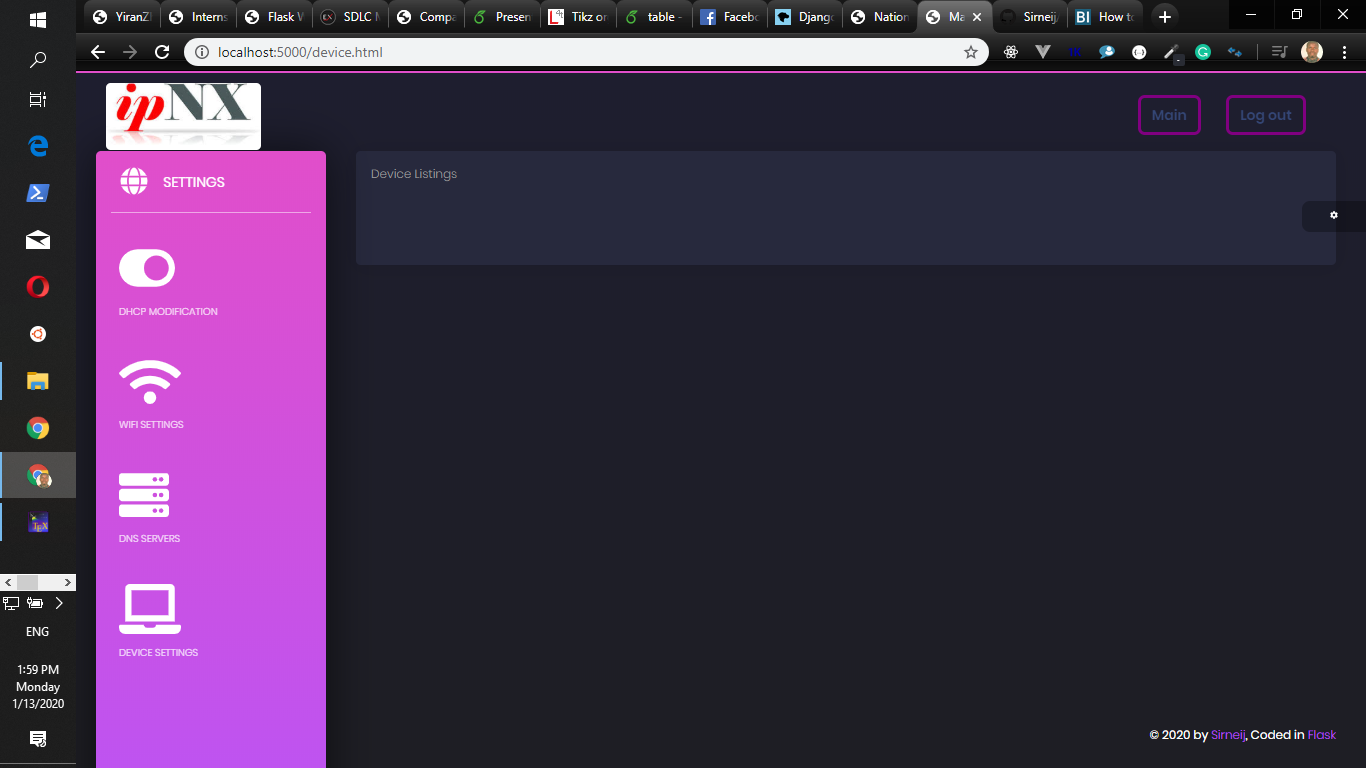
\includegraphics[width=\linewidth]{./vcpedevice}
	\caption{\ac{vCPE}  Devices List page}
\end{subfigure}
\medskip
\begin{subfigure}[b]{0.45\textwidth}
	\centering
	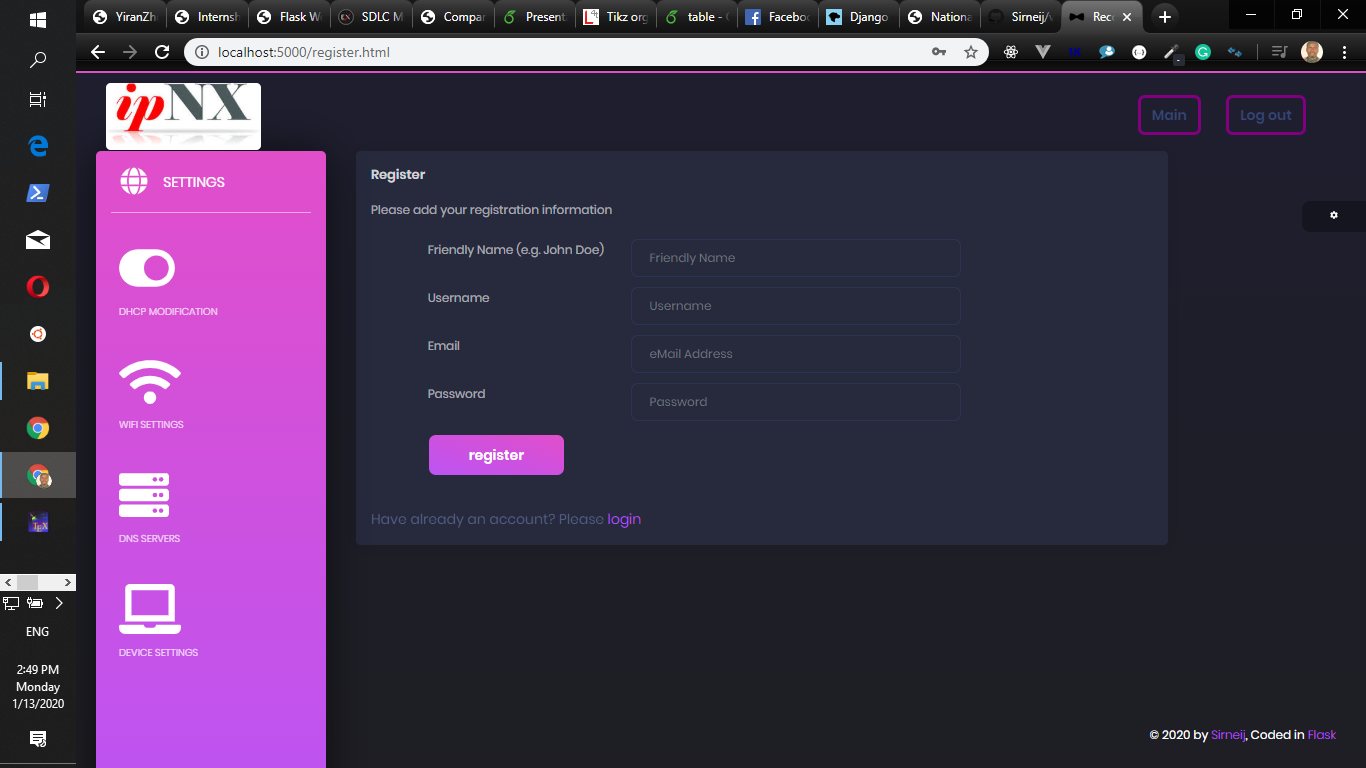
\includegraphics[width=\linewidth]{./vcperegister}
	\caption{\ac{vCPE} Registration page, \textit{restricted to an admin}.}
\end{subfigure}\hfill
\begin{subfigure}[b]{0.45\textwidth}
	\centering
	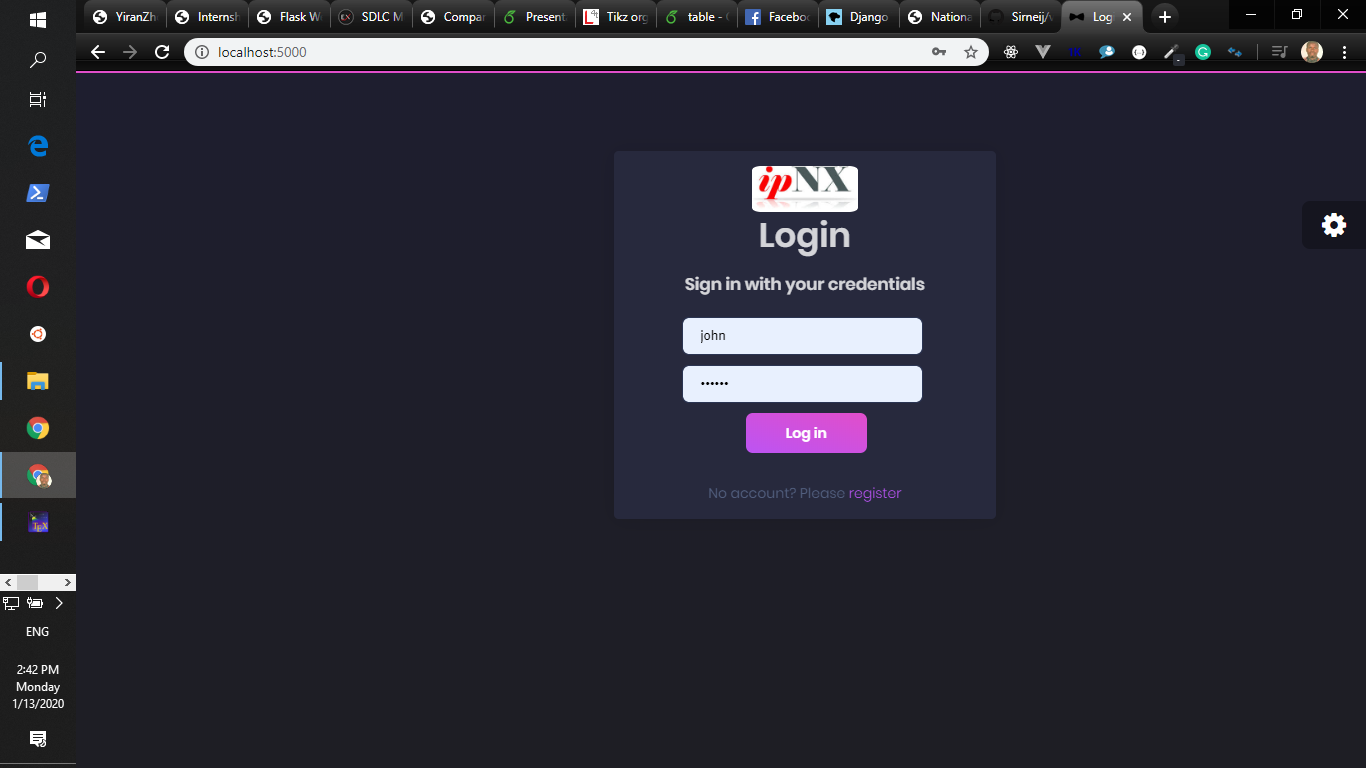
\includegraphics[width=\linewidth]{./vcpelogin}
	\caption{\ac{vCPE} Login page}
\end{subfigure}
	\caption{\ac{vCPE} Screenshots}
\end{figure}
\subsection{Customer Experience Analysis (CEA) Dashboard}
\begin{itemize}
	\item \textbf{Project's Requirement specification}: Customer Experience Analysis (CEA) Dashboard's requirement specification was to develop or implement a real-time dashboard which has the metrics and features as shown in the Figure 3.5 below:\\\\\\\\
	\begin{figure}[!htbp]
		\centering
		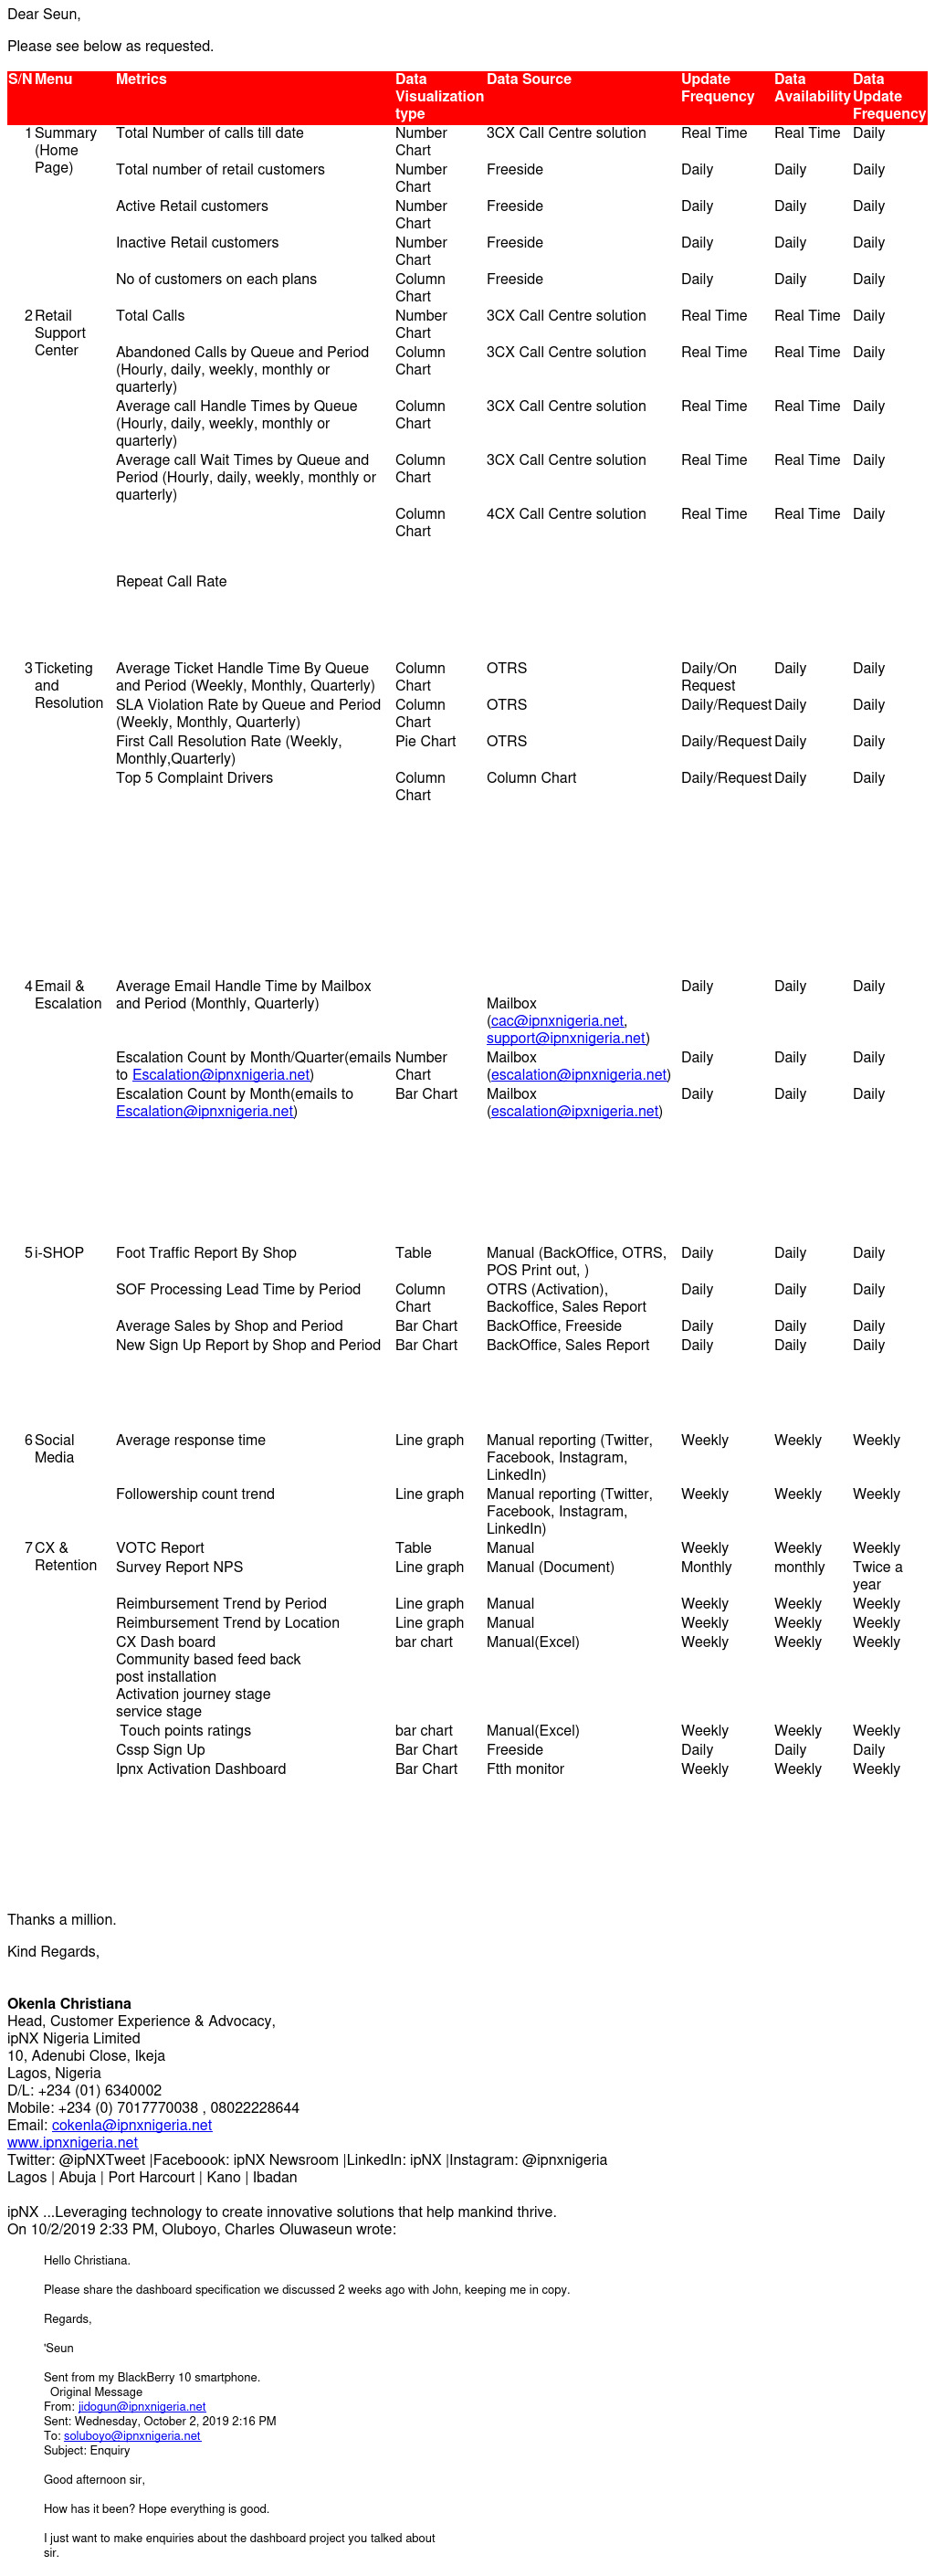
\includegraphics[width=1\linewidth,height=0.9\textheight]{./ceadash}
		\caption{Customer Experience Analysis (CEA) Dashboard specification sent by \textit{ip}NX's Head of Customer Experience \& Advocacy.}
	\end{figure}
	Figure 3.6 depicts the looks of the software product which was wholly implemented in Python's Flask:
	\begin{figure}[!htbp]
		\centering
		\begin{subfigure}[b]{0.45\textwidth}
			\centering
			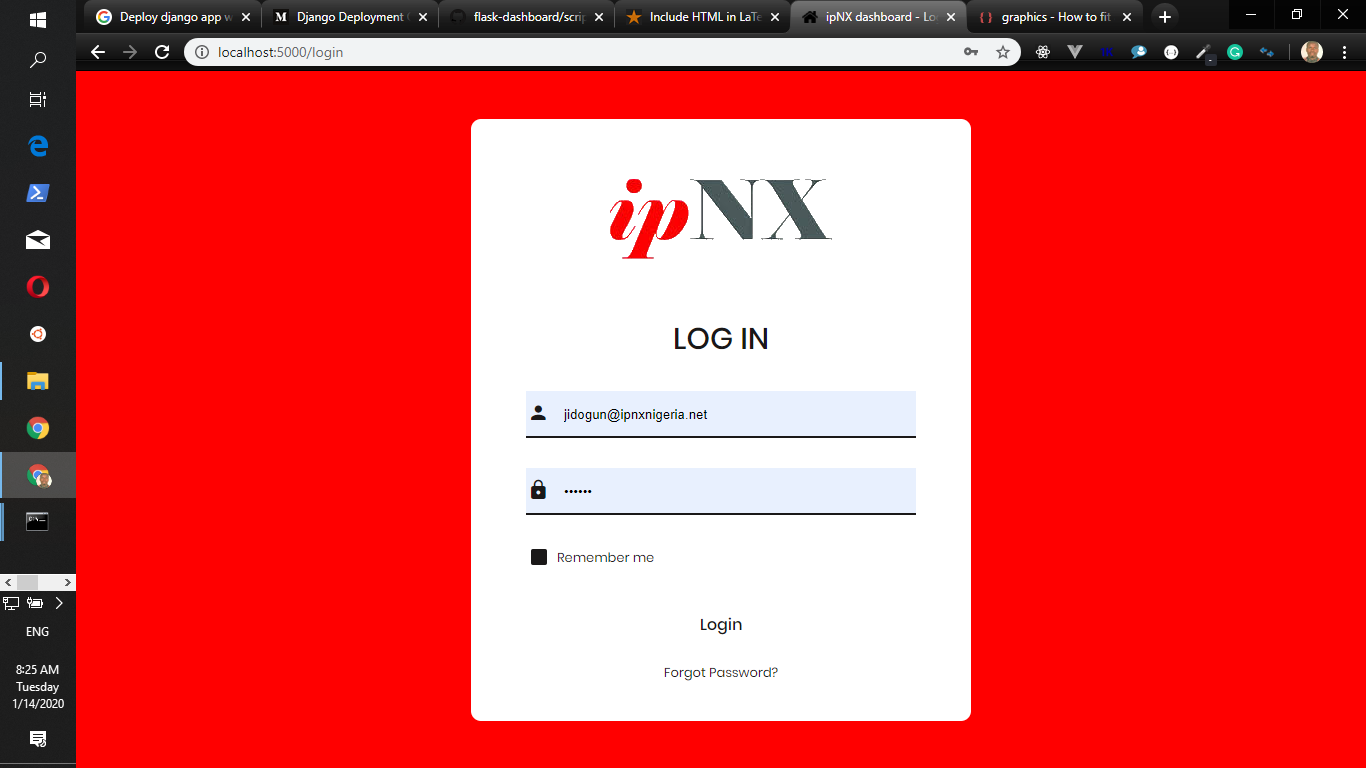
\includegraphics[width=\linewidth]{./cealogin}
			\caption{CEA dashboard Login page}
		\end{subfigure}
		\hfill
		\begin{subfigure}[b]{0.45\textwidth}
			\centering
			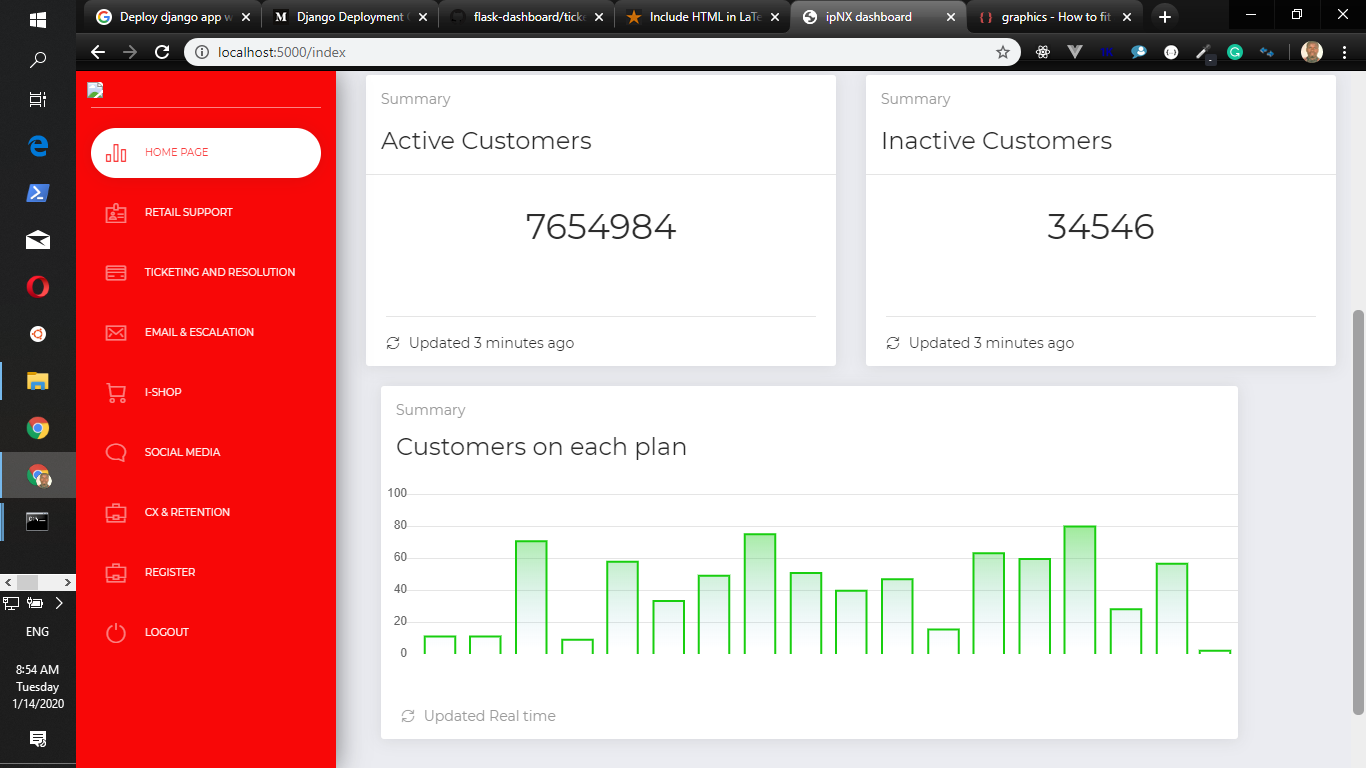
\includegraphics[width=\linewidth]{./ceaindex}
			\caption{CEA dashboard Landing or main page}
		\end{subfigure}
		\medskip
		\begin{subfigure}[b]{0.45\textwidth}
			\centering
			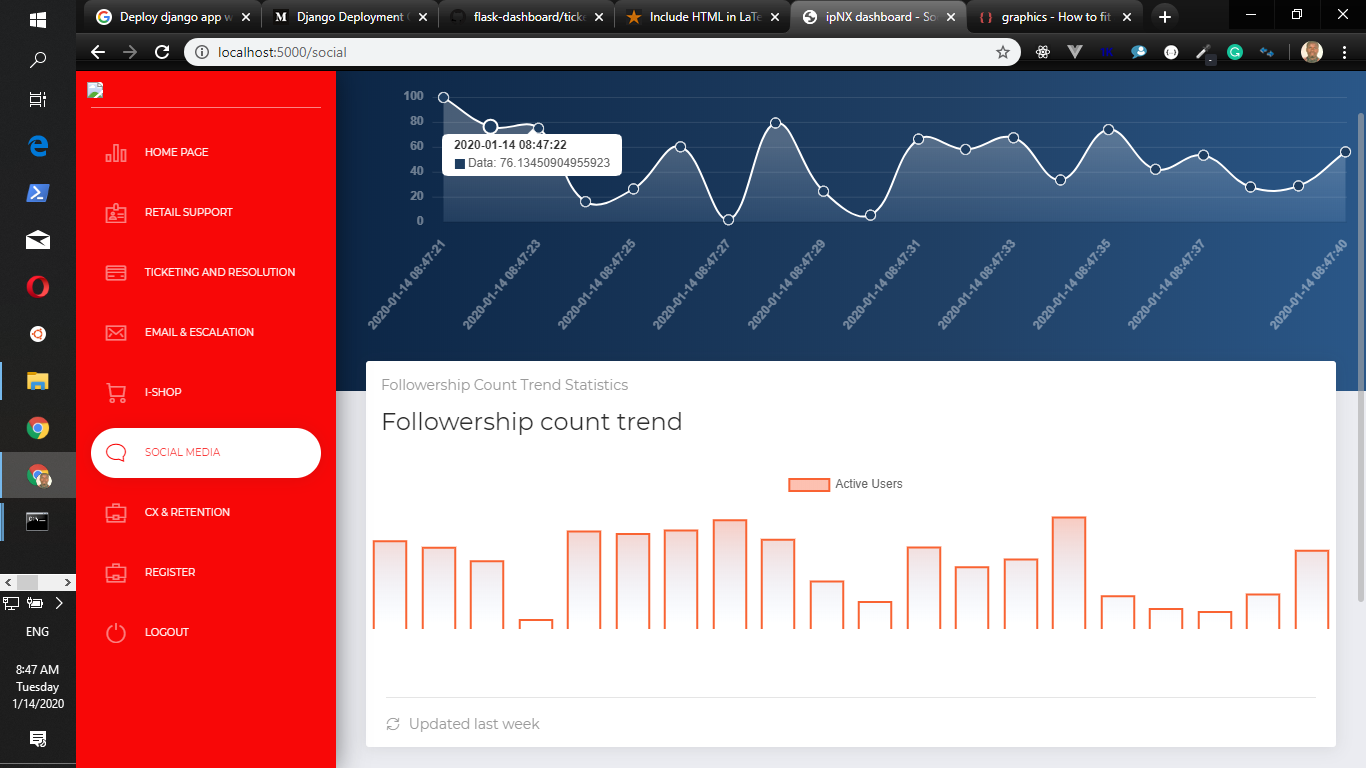
\includegraphics[width=\linewidth]{./ceasocial}
			\caption{CEA dashboard Social menu page}
		\end{subfigure}
		\hfill
		\begin{subfigure}[b]{0.45\textwidth}
			\centering
			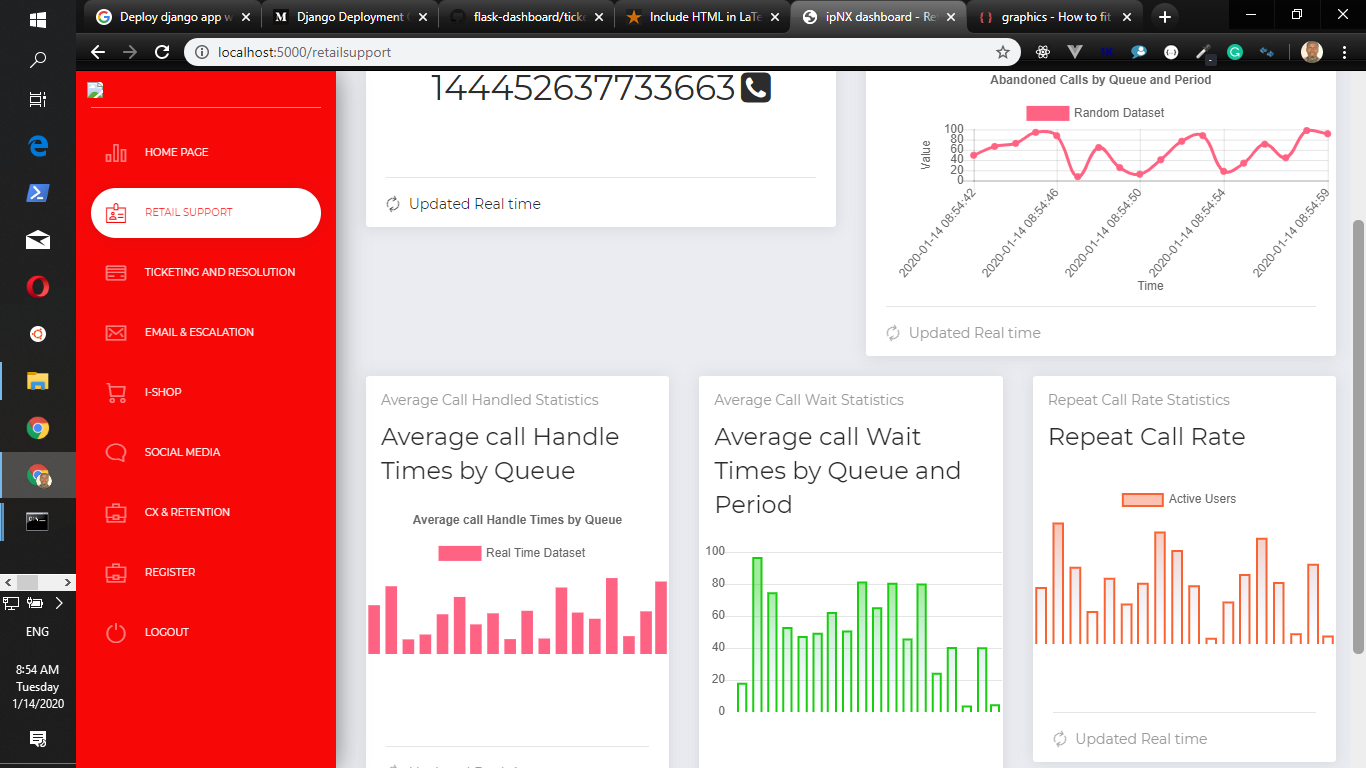
\includegraphics[width=\linewidth]{./cearetail}
			\caption{CEA dashboard Retail menu page}
		\end{subfigure}
		\caption{Some CEA dashboard pages with Real-time data visualization.}
	\end{figure}
\end{itemize}
\subsection{Data Usage Analytic (DUA) Dashboard}
\begin{itemize}
	\item \textbf{Project's requirement specification}: \textit{ip}NX already had a Data Usage Analytic (DUA) Dashboard but was with poor design and user interface. The task was to re-engineer, re-develop and revamp the whole system with the following additional features:
	\subitem Animated Error page for advertisement.
	\subitem Modal views of preliminary Data Usage analysis of each device on each user's network.
	\subitem Attractive Login page with company's products advertisement as carousels.
	\subitem Responsive Dashboard theme selection pluggin.\\
	
	
	 Figures 3.7 and 3.8 show the initial system as well as its re-designed, using Flask micro-framework, counterpart.
		\begin{figure}[!htbp]
		\centering
		\begin{subfigure}[b]{0.45\textwidth}
			\centering
			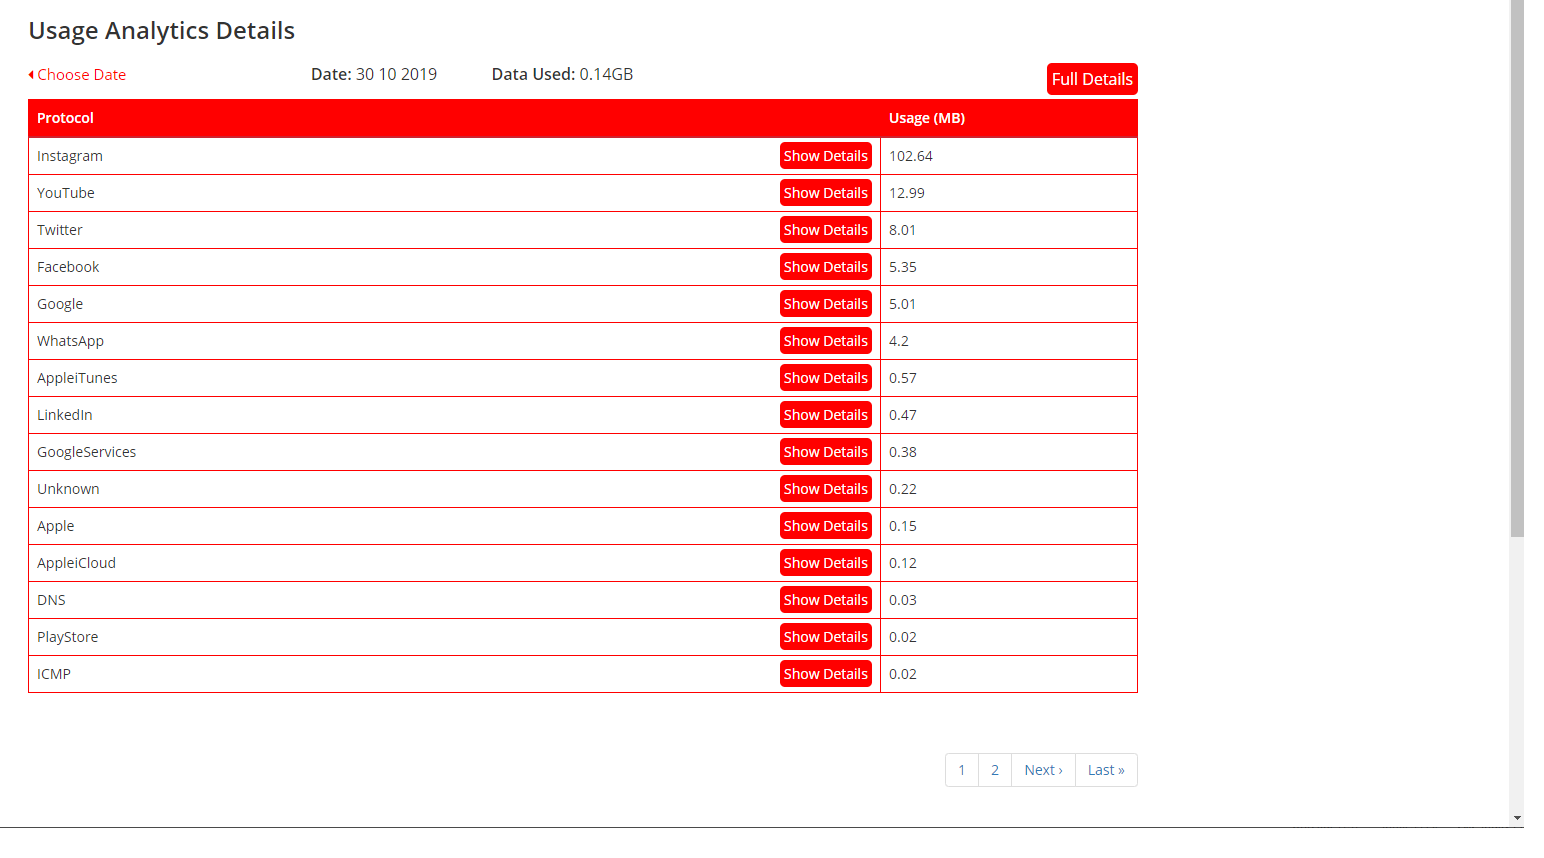
\includegraphics[width=\linewidth]{./duaformeranalytic}
			\caption{DUA dashboard data analytics}
		\end{subfigure}
		\hfill
		\begin{subfigure}[b]{0.45\textwidth}
			\centering
			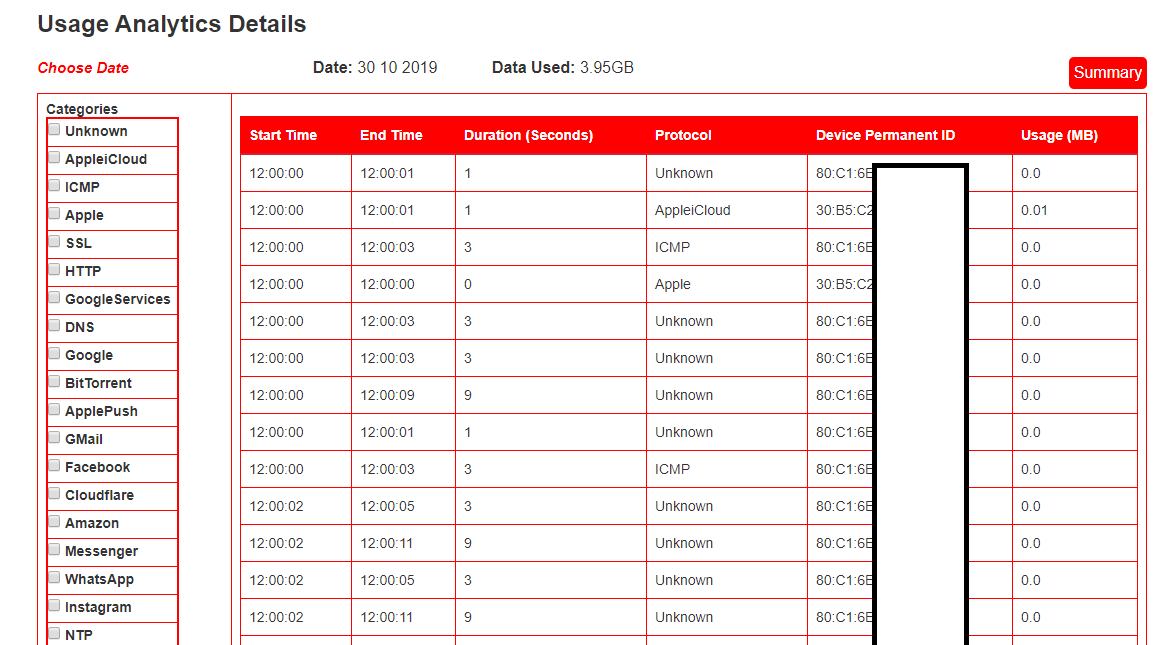
\includegraphics[width=\linewidth]{./duaformeranalyticdetail}
			\caption{DUA dashboard data analytics details}
		\end{subfigure}
		\caption{Former DUA dashboard pages.}
	\end{figure}
	\begin{figure}[!htbp]
		\centering
		\begin{subfigure}[b]{0.45\textwidth}
			\centering
			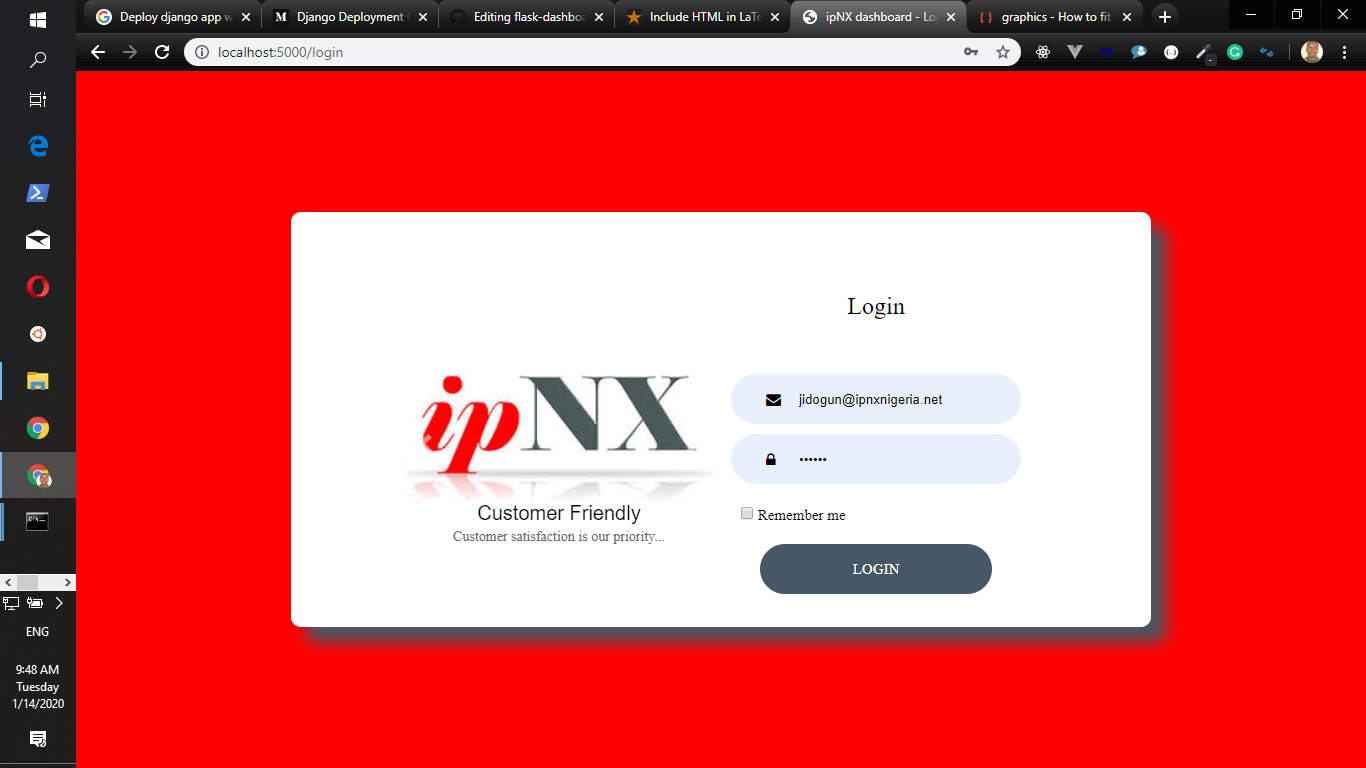
\includegraphics[width=\linewidth]{./dualogin}
			\caption{DUA dashboard Animated Login page}
		\end{subfigure}
		\hfill
		\begin{subfigure}[b]{0.45\textwidth}
			\centering
			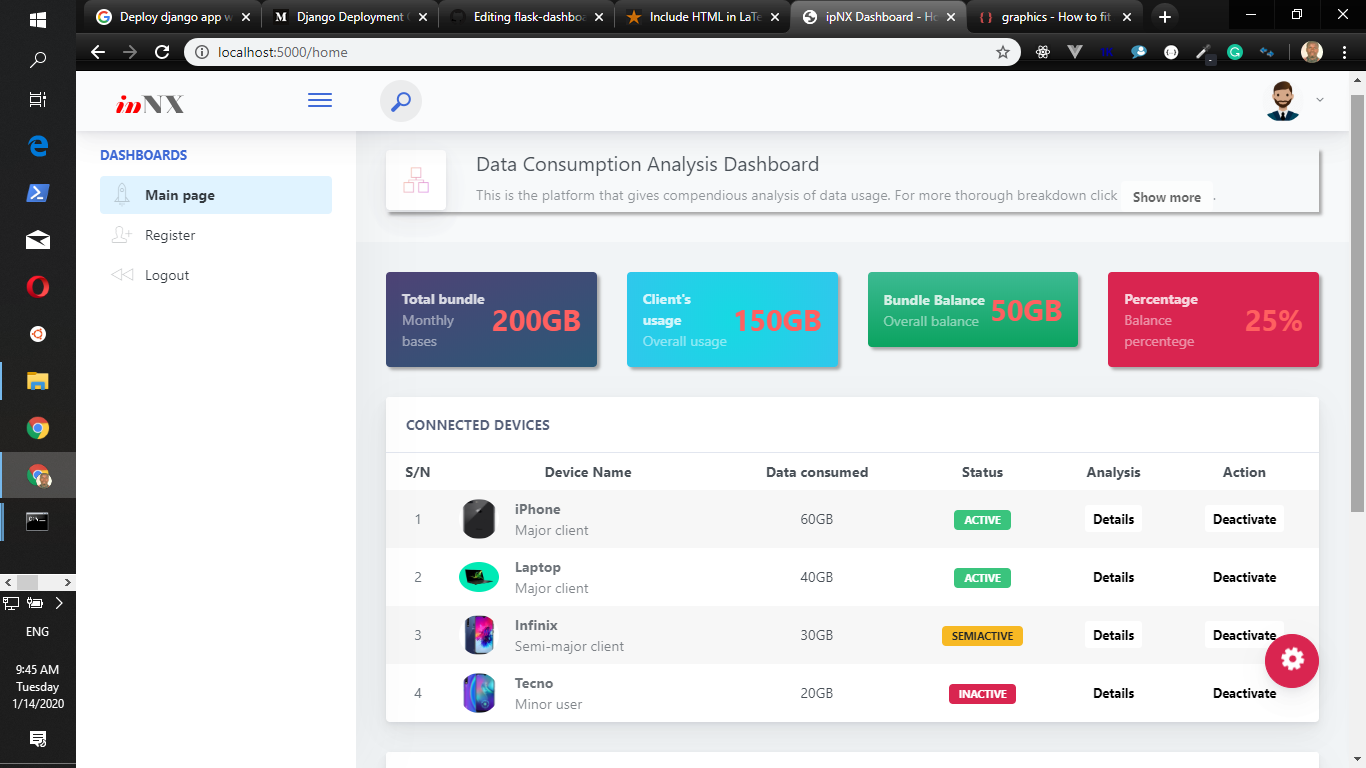
\includegraphics[width=\linewidth]{./duadata}
			\caption{DUA dashboard data analysis page}
		\end{subfigure}
	\medskip
	\begin{subfigure}[b]{0.45\textwidth}
		\centering
		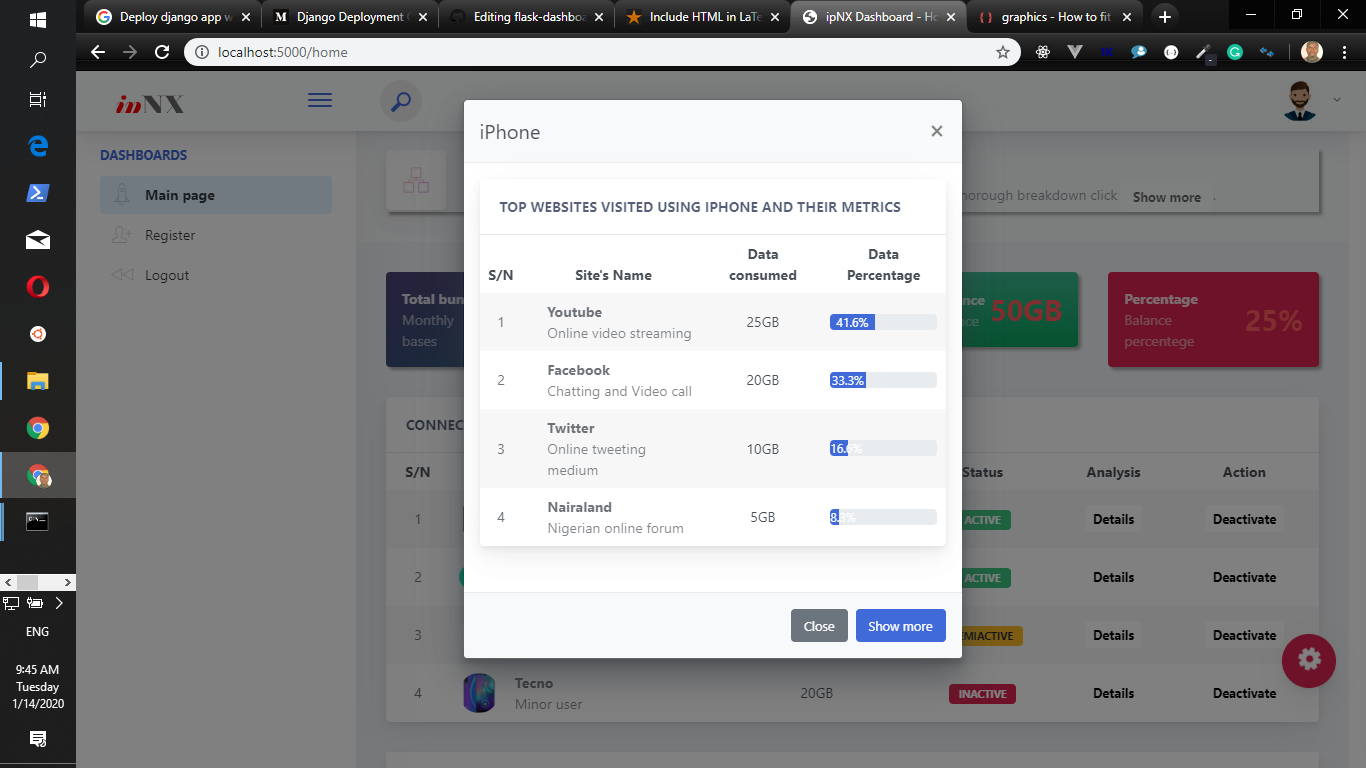
\includegraphics[width=\linewidth]{./duamodal}
		\caption{DUA dashboard modal data analysis page}
	\end{subfigure}
	\hfill
	\begin{subfigure}[b]{0.45\textwidth}
		\centering
		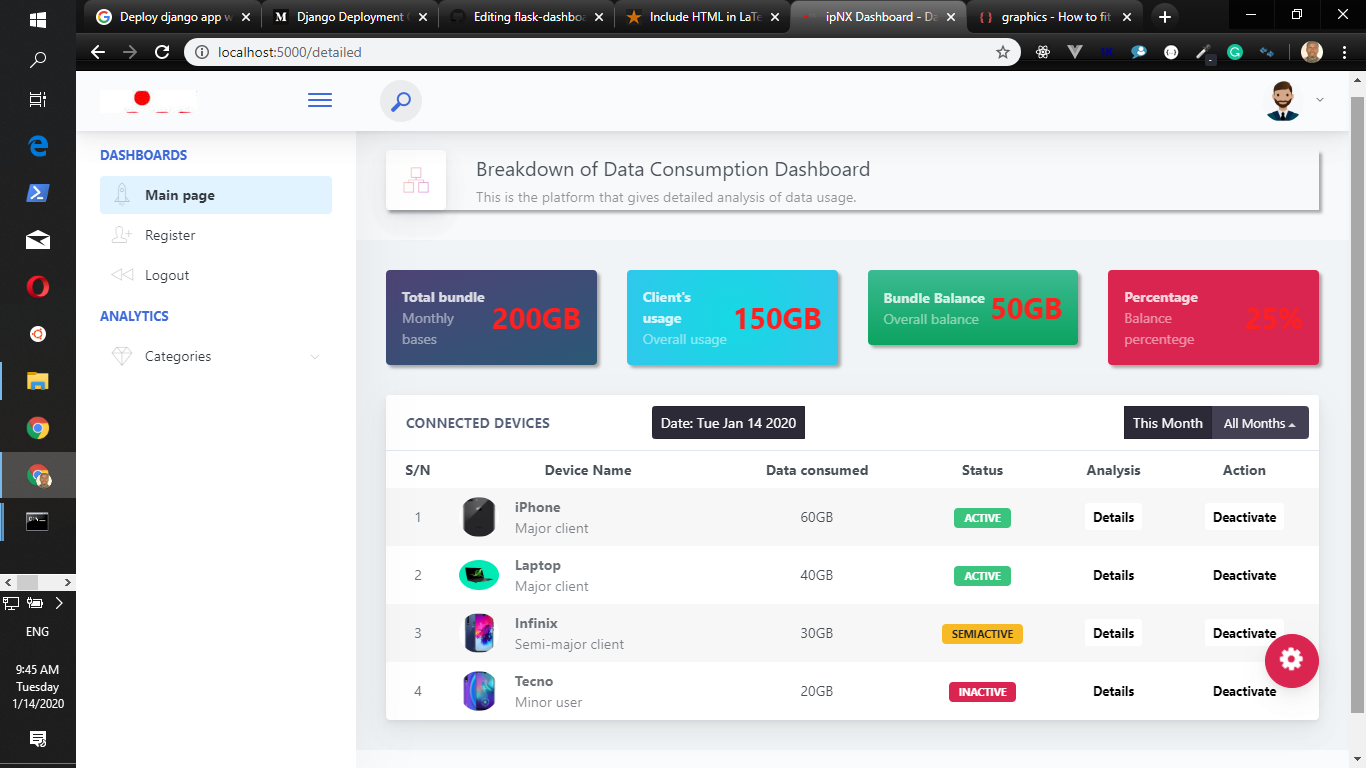
\includegraphics[width=\linewidth]{./duadatadetails}
		\caption{DUA dashboard detailed data analysis page}
	\end{subfigure}
	\medskip
	\begin{subfigure}[b]{0.5\textwidth}
		\centering
		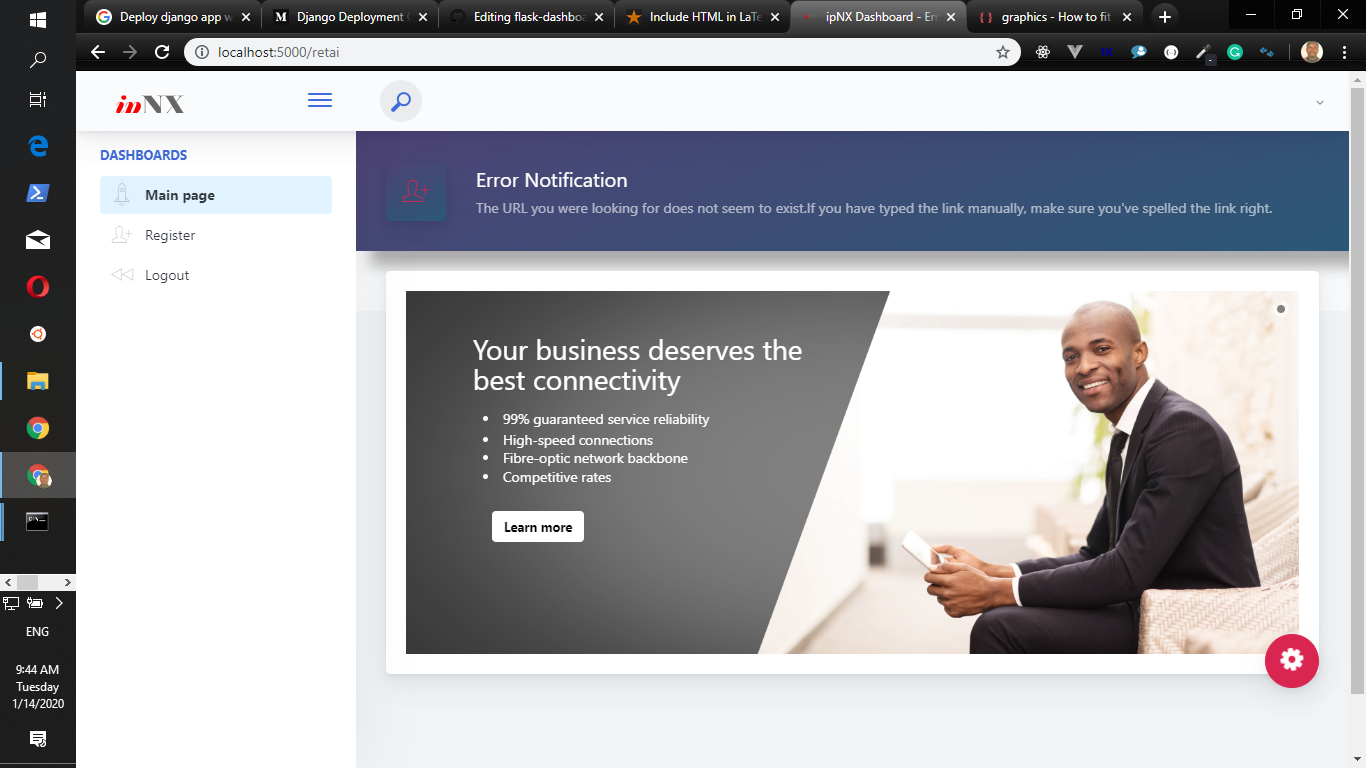
\includegraphics[width=\linewidth]{./duaerror}
		\caption{DUA dashboard Animated Error page}
	\end{subfigure}
		\caption{Re-designed DUA dashboard pages.}
	\end{figure}
\end{itemize}
\subsection{Django Blog}
\begin{itemize}
	\item \textbf{Project's description}: \textbf{Devc}, the name of the blog, is a complex web application inspired by \textbf{Frances Nnamadim}, a senior and regular colleague who worked as a Business Analyst and \ac{UI}/\ac{UX} designer in \textit{ip}NX's department of Business Intelligence and Data Analytics (BIDA). It was fully implemented in Django framework with PostgreSQL database at the back-end and a template initially designed by \href{https://www.styleshout.com/}{Styleshout}.\\
	
	\textbf{Devc} was built with three (3) other main applications embedded, each embedding other systems in turn:
	\subitem \textbf{Account management system}: This application provides interfaces for users registration and authentication. It allows direct authentication from popular social and technical websites such as Facebook, Twitter and Github among others as shown in Figure 3.9.
	\begin{figure}[!htbp]
		\centering
		\begin{subfigure}[b]{0.45\textwidth}
			\centering
			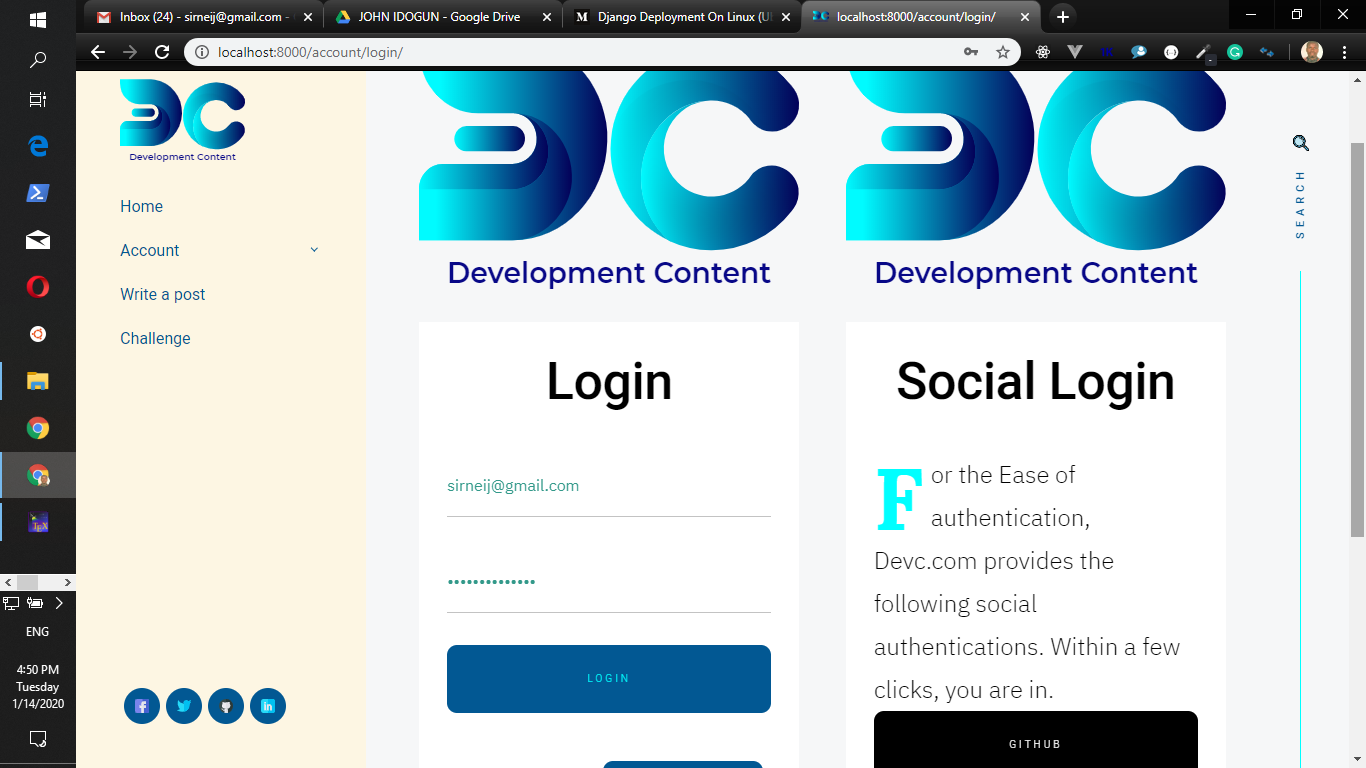
\includegraphics[width=\linewidth]{./devclogin}
			\caption{\textbf{devc} Login page with social authentication}
		\end{subfigure}
		\hfill
		\begin{subfigure}[b]{0.45\textwidth}
			\centering
			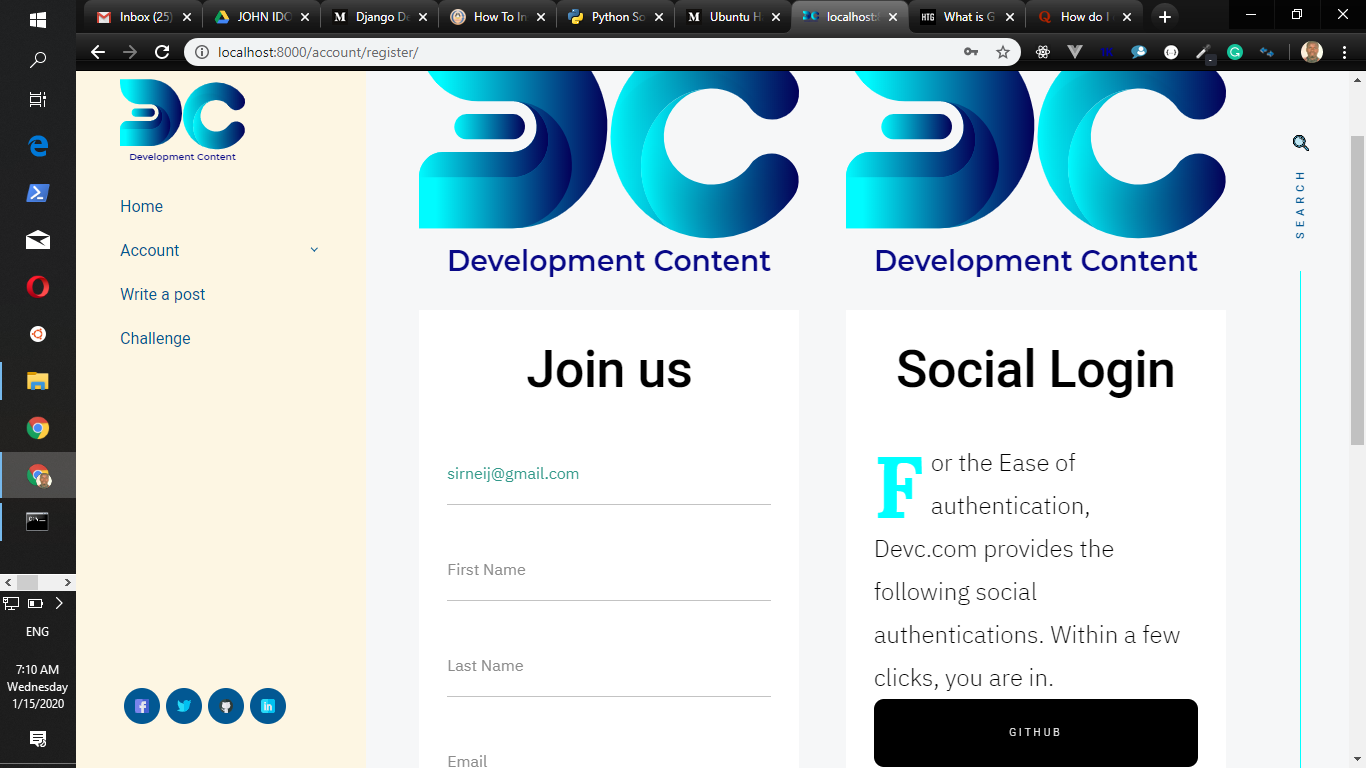
\includegraphics[width=\linewidth]{./devcsignup}
			\caption{\textbf{devc} Signup page with social authentication}
		\end{subfigure}
		\medskip
		\begin{subfigure}[b]{0.5\textwidth}
			\centering
			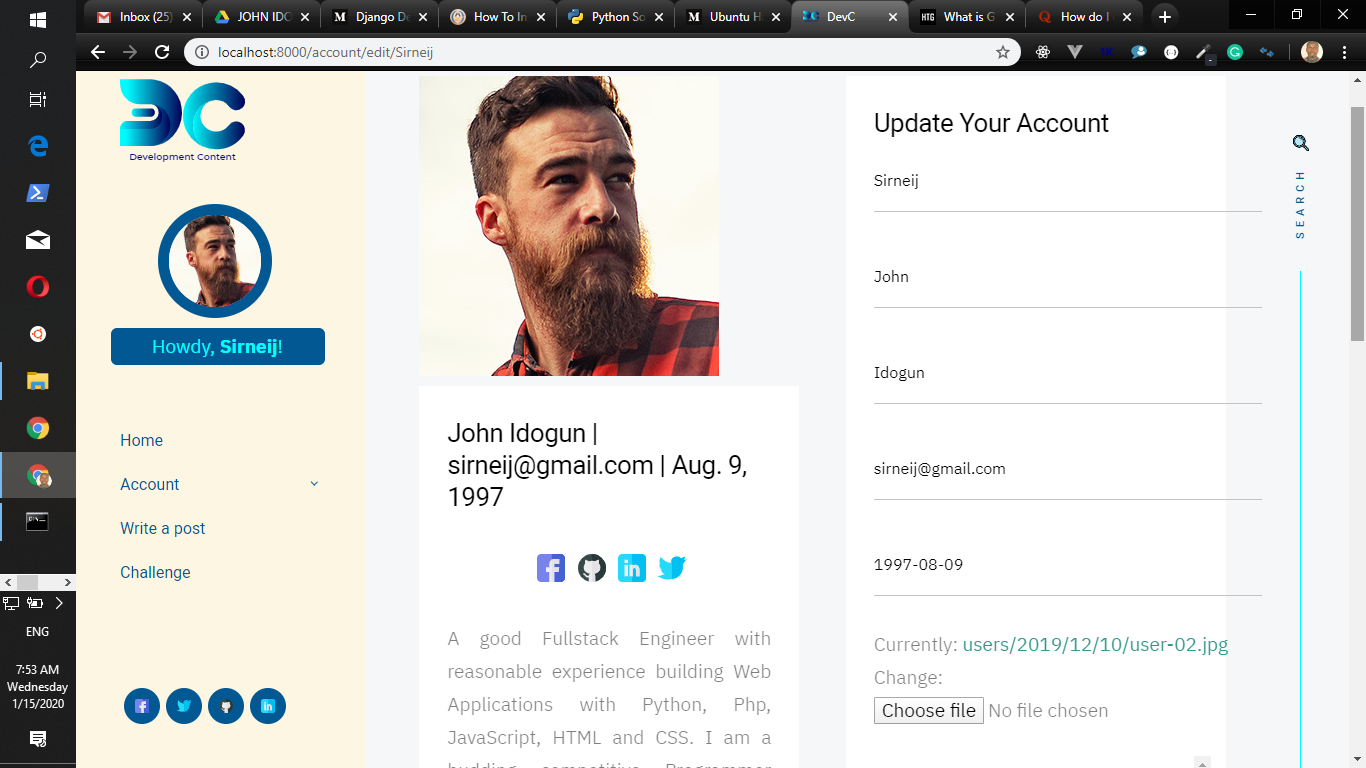
\includegraphics[width=\linewidth]{./devcaccount}
			\caption{\textbf{devc} Account update page}
		\end{subfigure}
		\caption{\textbf{devc} Account management system.}
	\end{figure}
	\subitem \textbf{Blogging system}: This is the heart of the overall system. It controls user's posts - their creation and  update, with a rich text editor and advanced text formatting system; and posts' deletion - profiles and portfolio with various mini-systems such as full-text search engine, tagging, related-posts recommendation, threaded commenting and slack-like chatting systems, embedded. Users' posts could also be liked and shared asynchronously. Some of these features are shown in Figure 3.10.
	\begin{figure}[!htbp]
		\centering
		\begin{subfigure}[b]{0.45\textwidth}
			\centering
			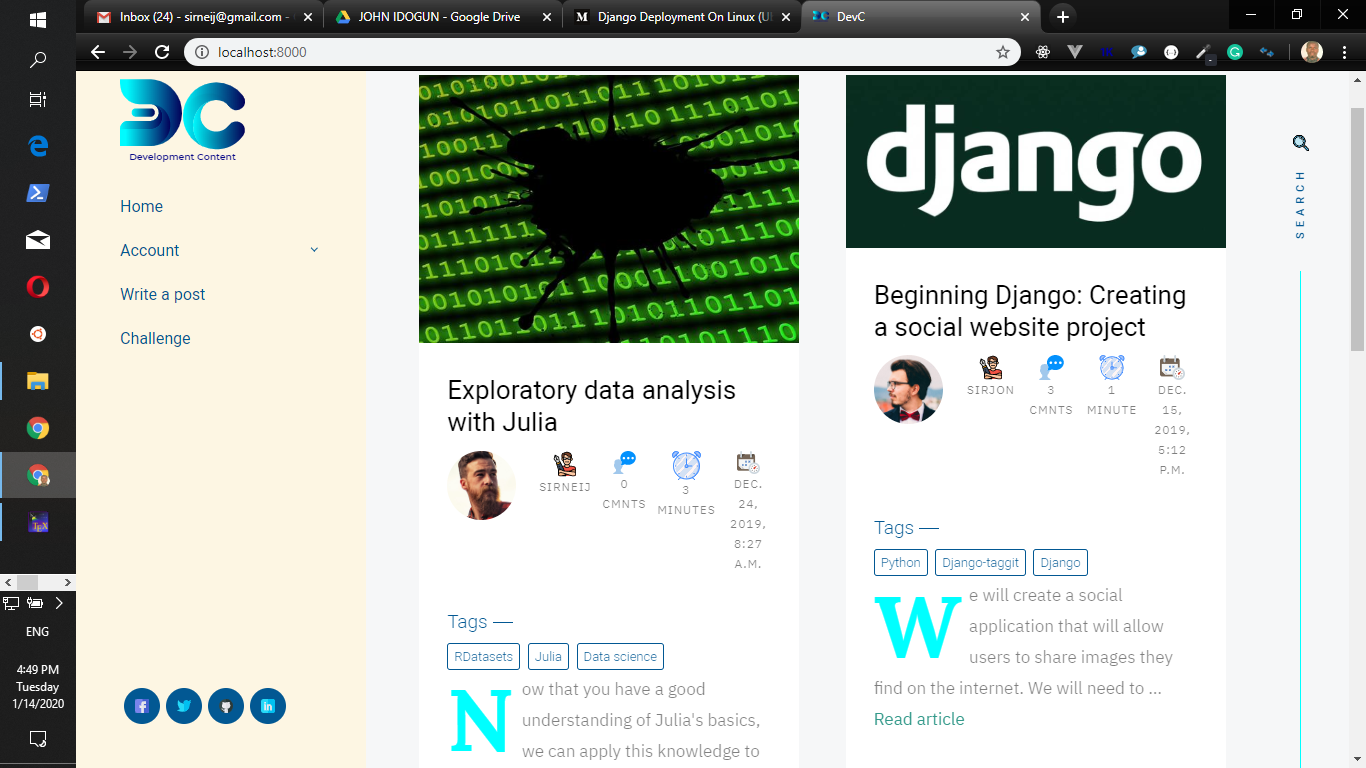
\includegraphics[width=\linewidth]{./devcmainwithout}
			\caption{\textbf{devc} main page without user authentication}
		\end{subfigure}
		\hfill
		\begin{subfigure}[b]{0.45\textwidth}
			\centering
			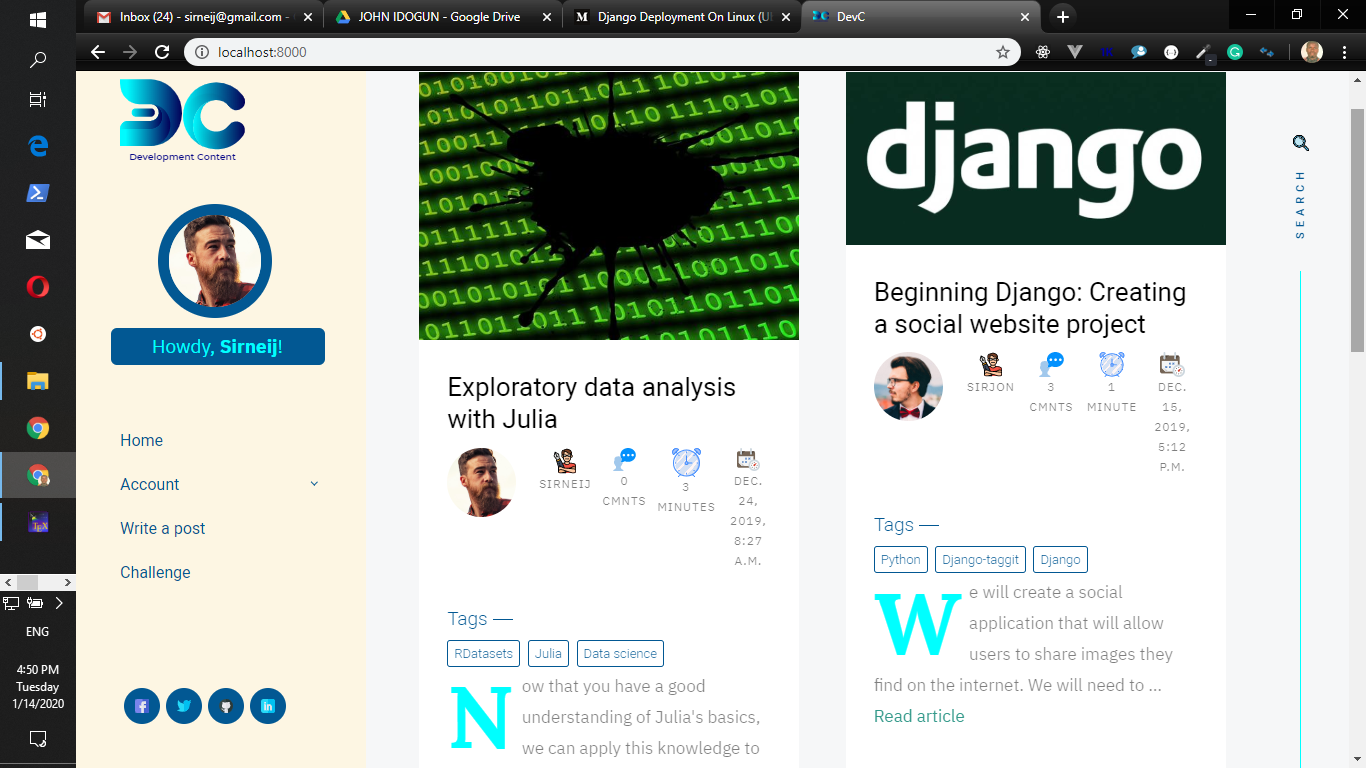
\includegraphics[width=\linewidth]{./devcmainwith}
			\caption{\textbf{devc} main page with user authentication, recent posts shown first.}
		\end{subfigure}
	\medskip
	\begin{subfigure}[b]{0.45\textwidth}
		\centering
		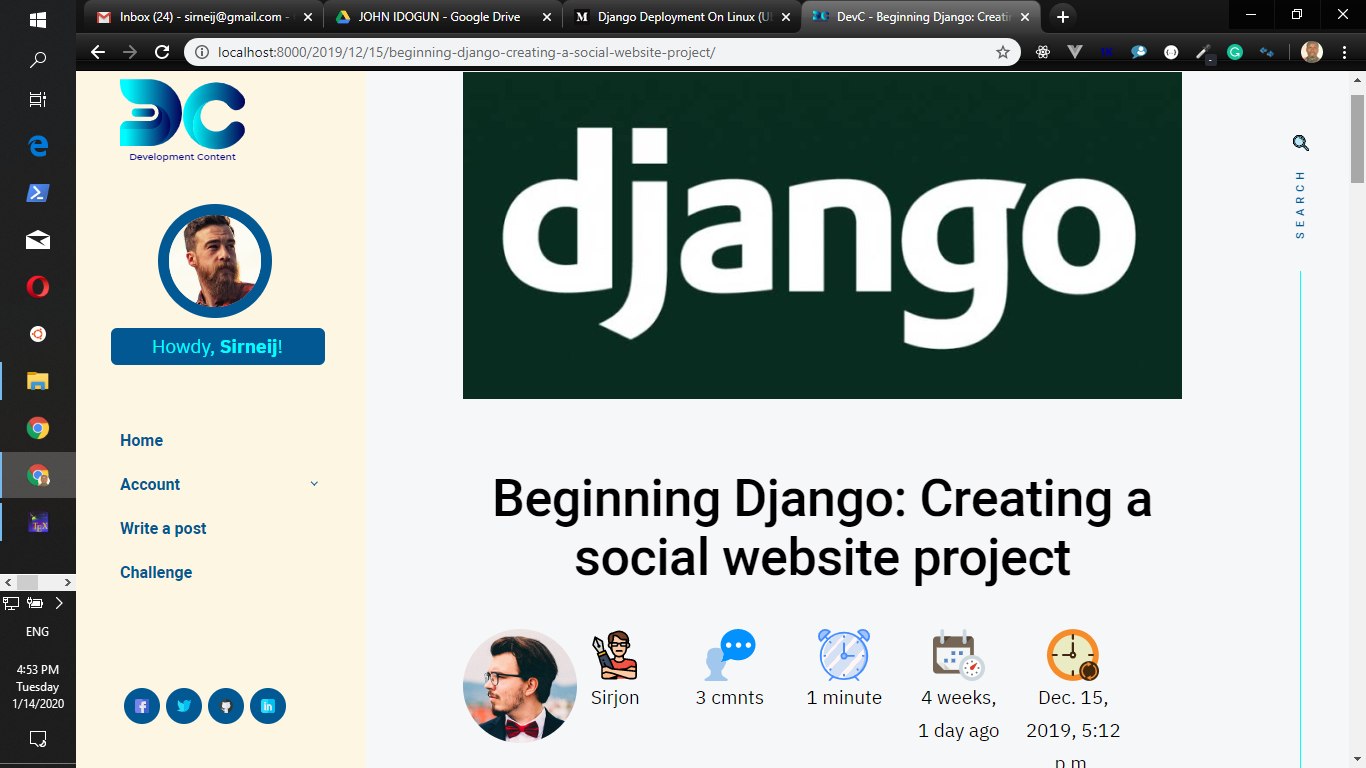
\includegraphics[width=\linewidth]{./devcpostdetail}
		\caption{\textbf{devc} Post detail page with user authentication}
	\end{subfigure}
	\hfill
	\begin{subfigure}[b]{0.45\textwidth}
		\centering
		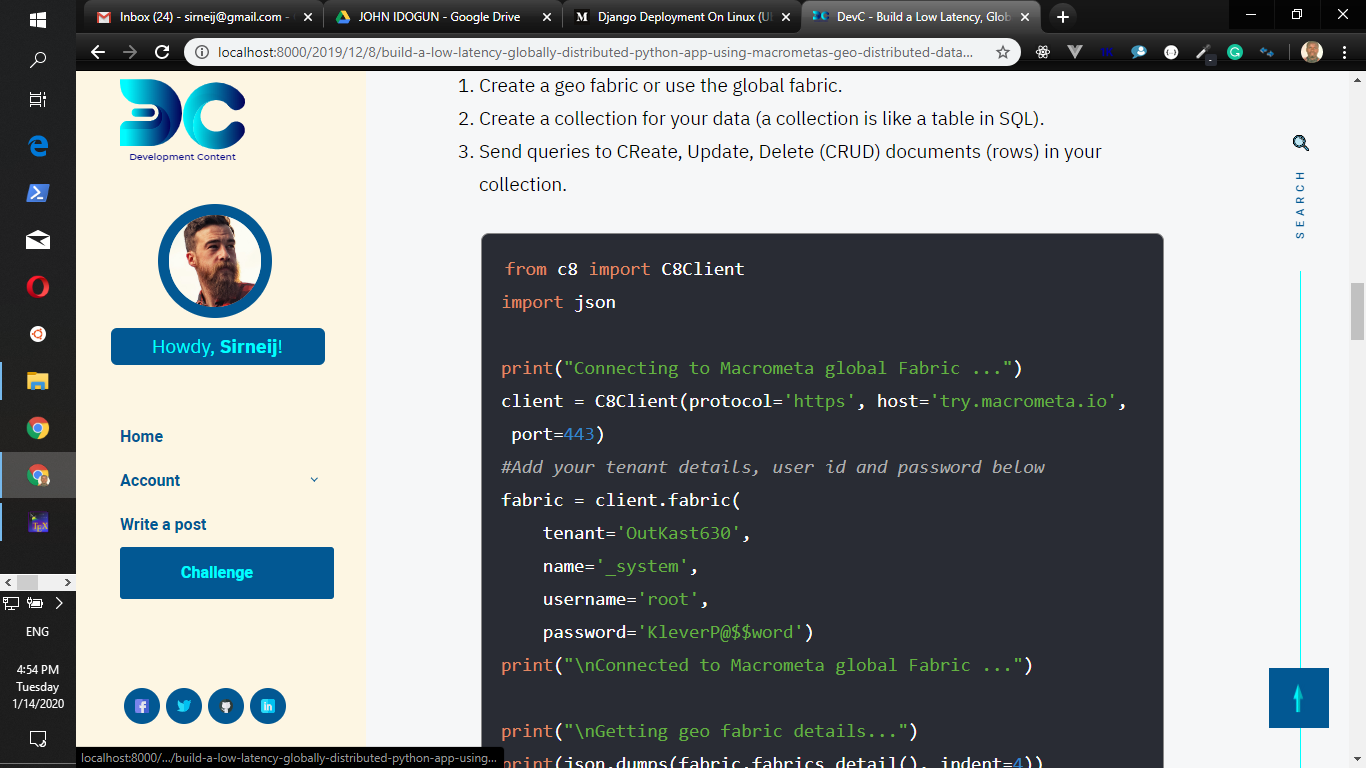
\includegraphics[width=\linewidth]{./devcpostdetailwith}
		\caption{\textbf{devc} syntax highlighting feature of the post detail page}
	\end{subfigure}
	\medskip
	\begin{subfigure}[b]{0.45\textwidth}
		\centering
		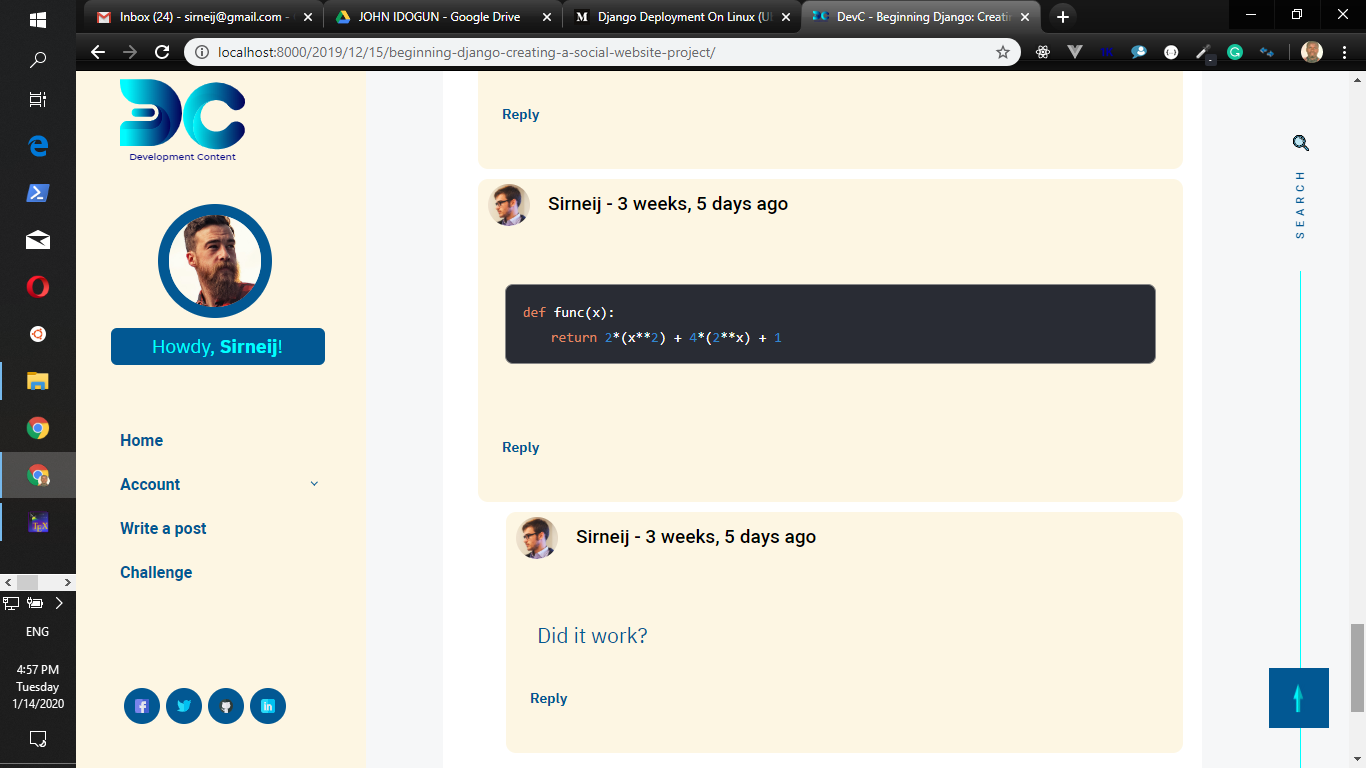
\includegraphics[width=\linewidth]{./devccomments}
		\caption{\textbf{devc} Threaded commenting section of the post detail page}
	\end{subfigure}
	\hfill
	\begin{subfigure}[b]{0.45\textwidth}
		\centering
		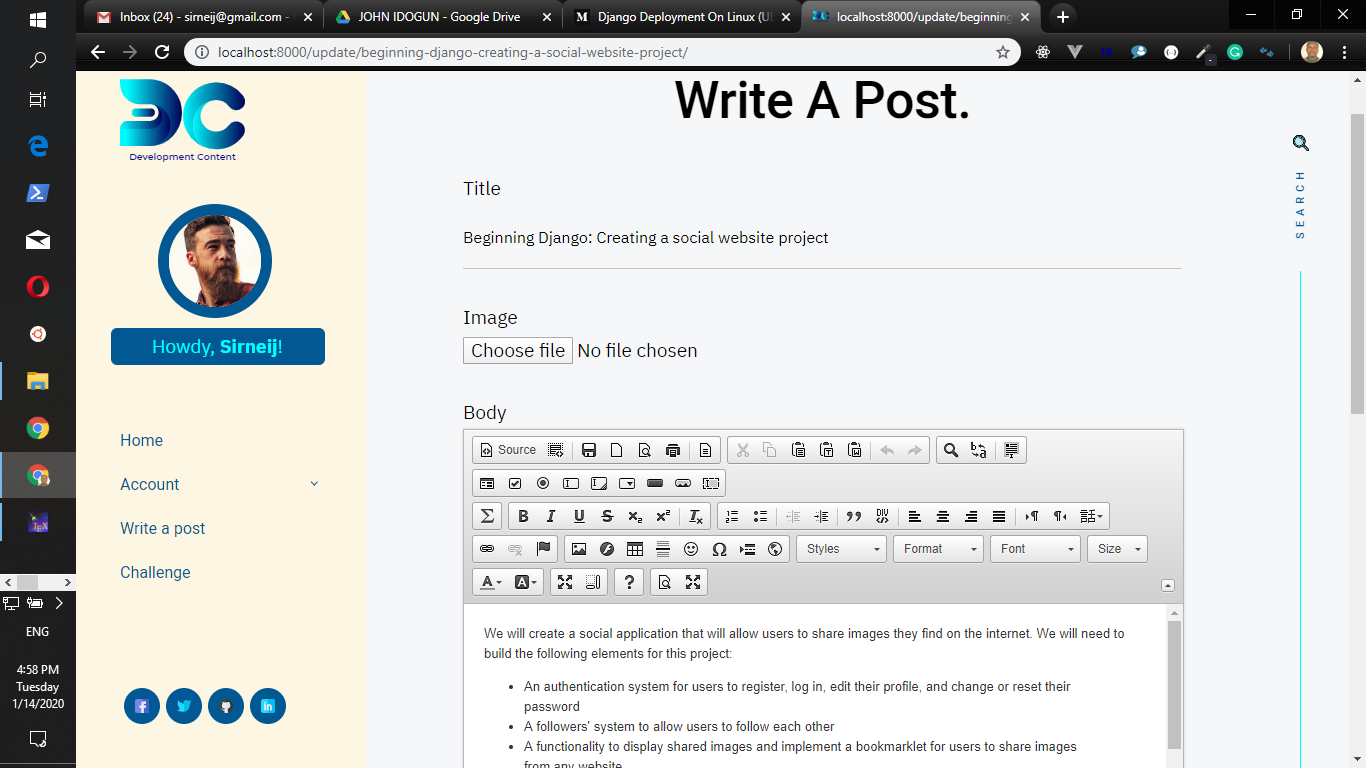
\includegraphics[width=\linewidth]{./devcpostupdate}
		\caption{\textbf{devc} post creation and update page with a Rich text editor}
	\end{subfigure}
		\caption{\textbf{devc} Blogging system.}
	\end{figure}
	\subitem \textbf{Portfolio system}: This serves as an extension of the account management system where authors of post(s) showcase their skills to their potential recruiters. It structures authors profiles, education, skills, projects and recommendations accordingly which can be downloaded in Portable Document Format (PDF). Figure 3.11 gives a quick tour of some of these features.
	\begin{figure}[!htbp]
		\centering
		\begin{subfigure}[b]{0.45\textwidth}
			\centering
			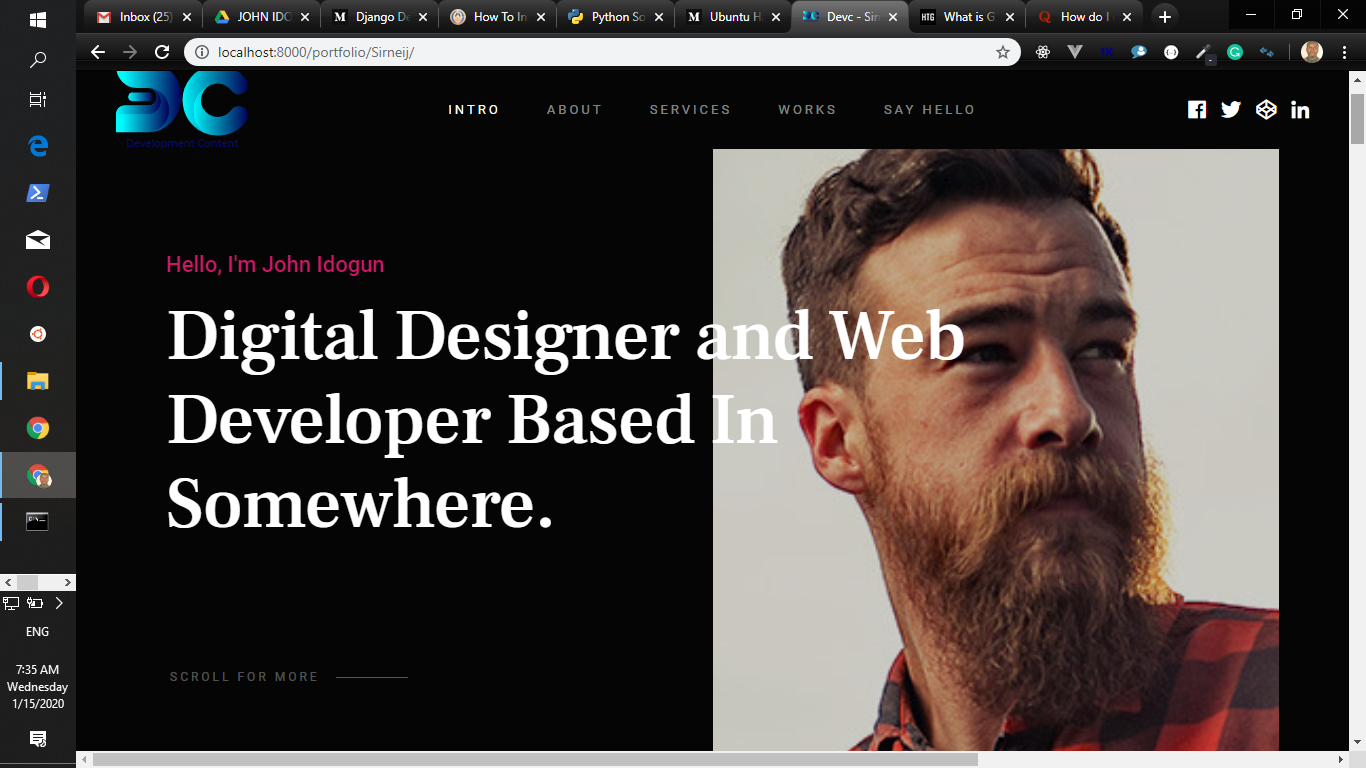
\includegraphics[width=\linewidth]{./devcportprofile}
			\caption{\textbf{devc} portfolio introduction section.}
		\end{subfigure}
		\hfill
		\begin{subfigure}[b]{0.45\textwidth}
			\centering
			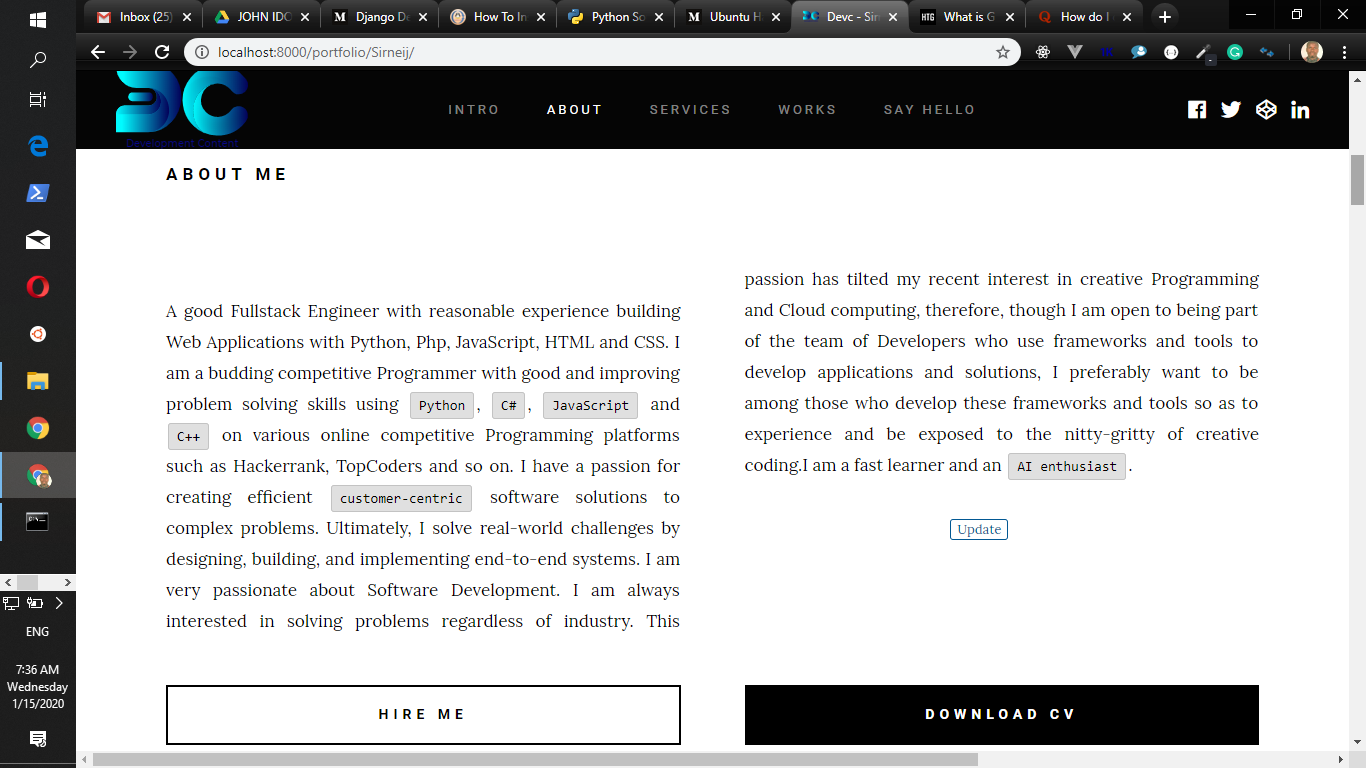
\includegraphics[width=\linewidth]{./devcportabout}
			\caption{\textbf{devc} portfolio about section.}
		\end{subfigure}
		\medskip
		\begin{subfigure}[b]{0.45\textwidth}
			\centering
			
\includegraphics[width=\linewidth]{./devcportwork}
			\caption{\textbf{devc} portfolio experience section}
		\end{subfigure}
		\hfill
		\begin{subfigure}[b]{0.45\textwidth}
			\centering
			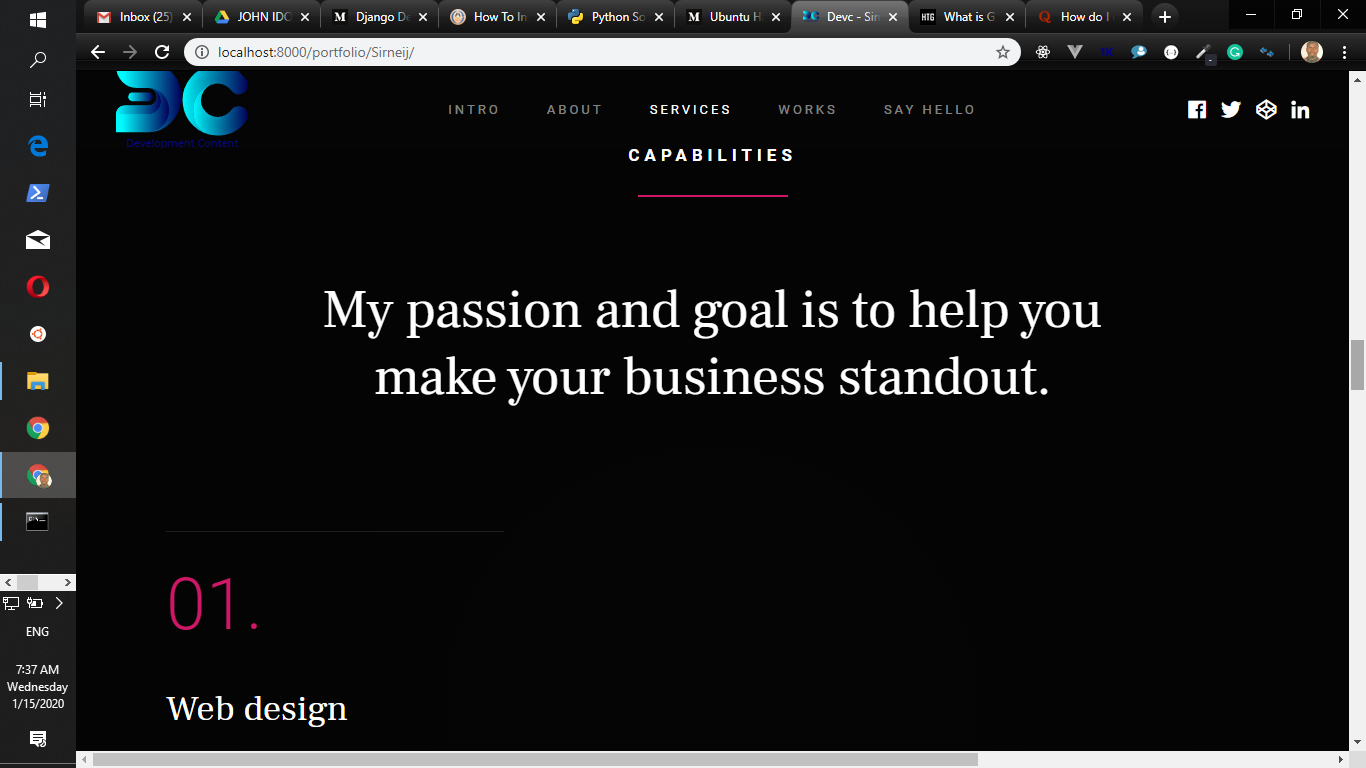
\includegraphics[width=\linewidth]{./devcportservices}
			\caption{\textbf{devc} portfolio service section}
		\end{subfigure}
		\medskip
		\begin{subfigure}[b]{0.45\textwidth}
			\centering
			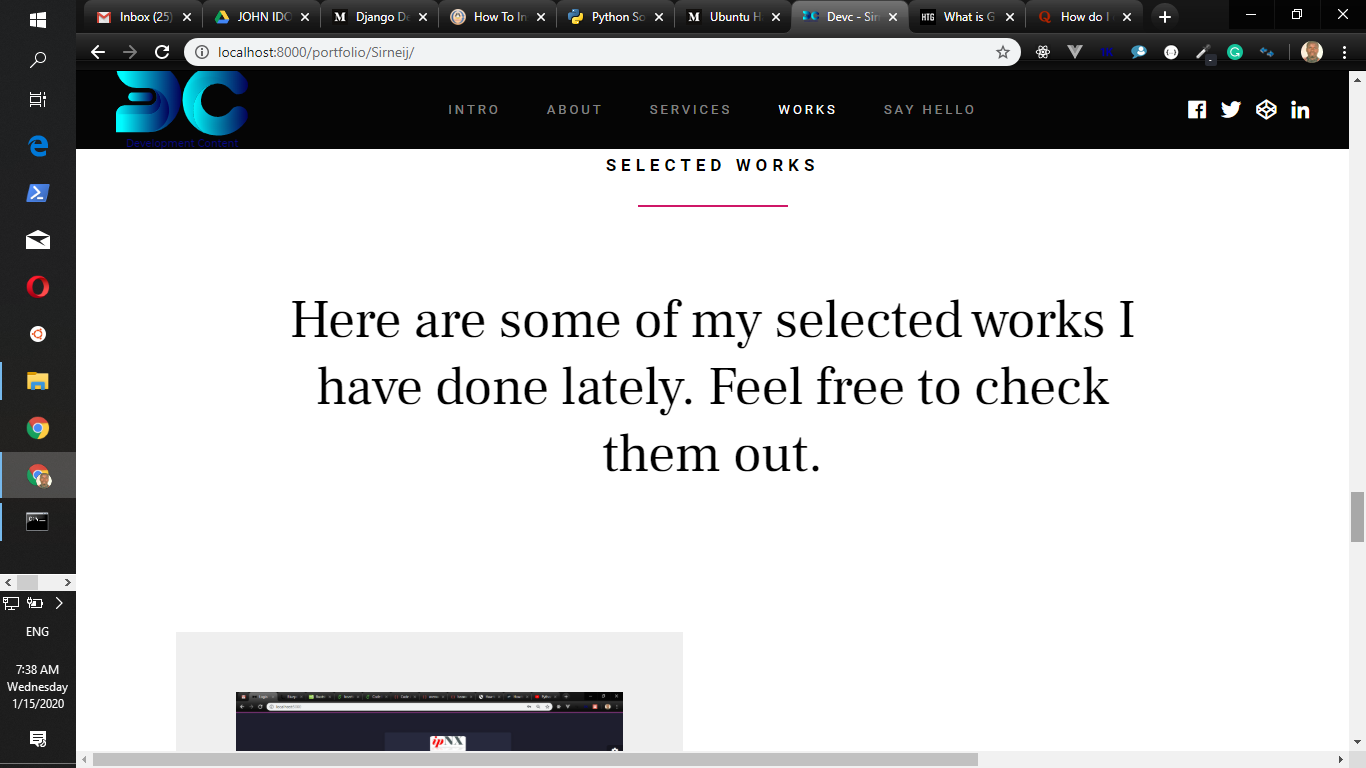
\includegraphics[width=\linewidth]{./devcportproject}
			\caption{\textbf{devc} portfolio project showcase section}
		\end{subfigure}
		\hfill
		\begin{subfigure}[b]{0.45\textwidth}
			\centering
			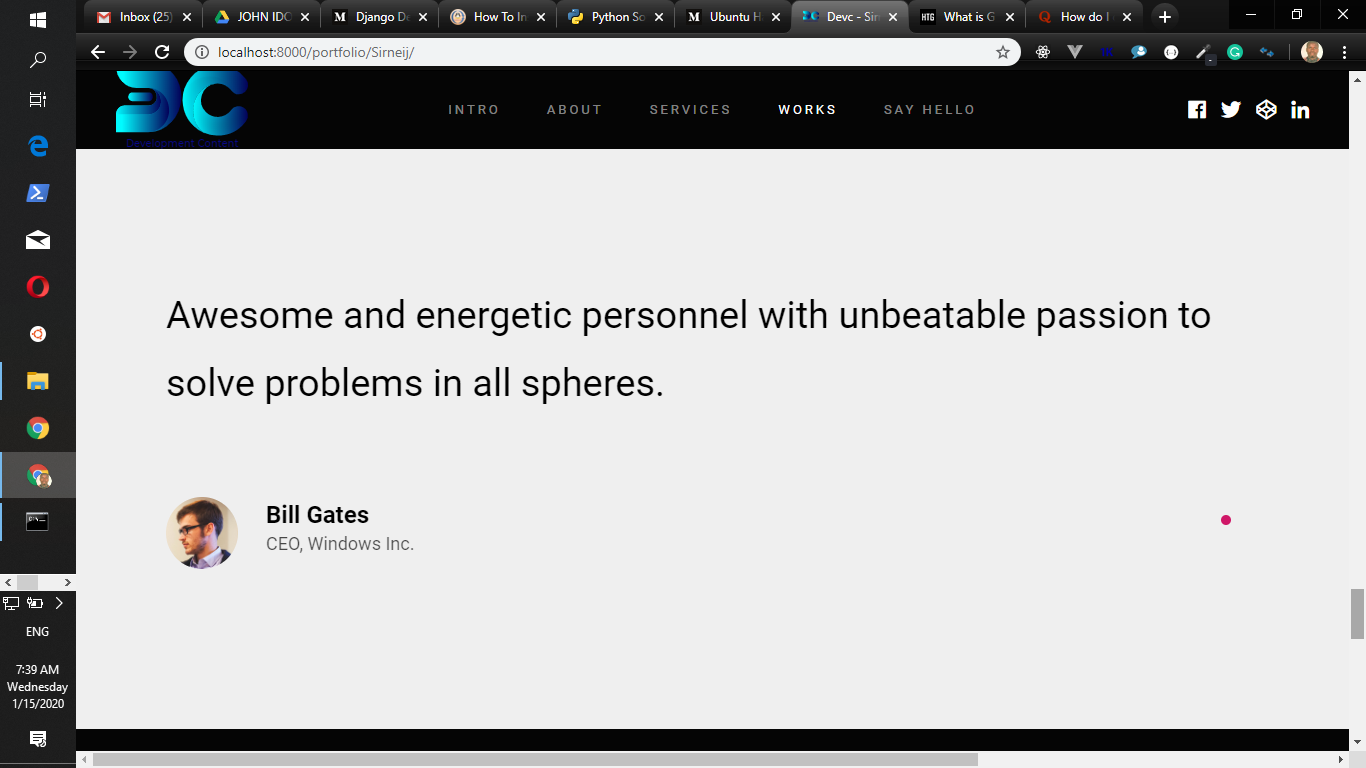
\includegraphics[width=\linewidth]{./devcportrecommend}
			\caption{\textbf{devc} portfolio recommendation section}
		\end{subfigure}
		\medskip
		\begin{subfigure}[b]{0.5\textwidth}
			\centering
			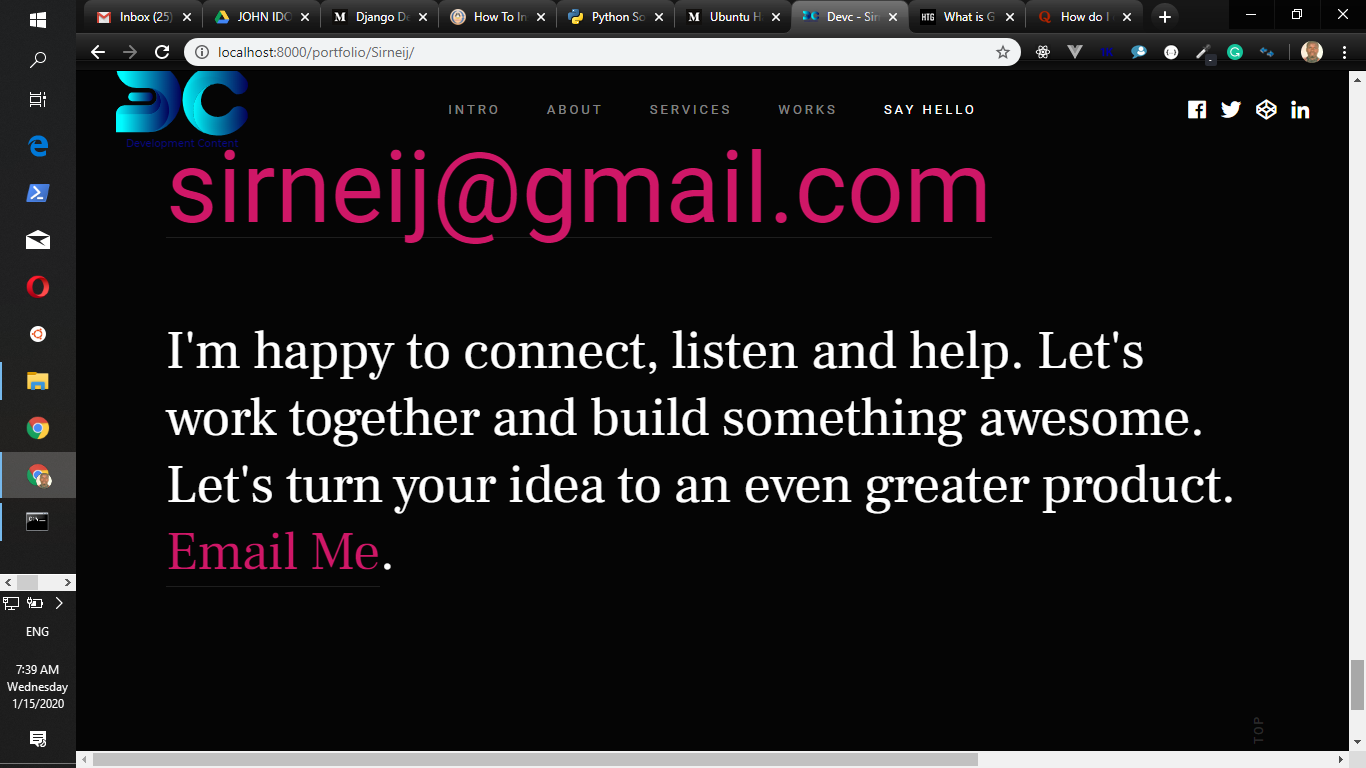
\includegraphics[width=\linewidth]{./devcportgetintouch}
			\caption{\textbf{devc} portfolio Get-in-touch section}
		\end{subfigure}
		\caption{\textbf{devc} Portfolio system.}
	\end{figure}
\end{itemize}
\subsection{Web Crawler}
\subsection{Recommender System}
\subsection{Deployment}
